\documentclass{book}
\usepackage[a4paper, margin=1in]{geometry}
\usepackage{amsmath,amsfonts,amssymb}
\usepackage{graphicx}
\usepackage{float}
%---------------------
\usepackage[numbers, square]{natbib}
\usepackage{fancyhdr}
\pagestyle{fancy}
\fancyhf{}
\fancyfoot[C]{\thepage}
\renewcommand{\headrulewidth}{0pt}
\renewcommand{\footrulewidth}{0pt}
%-----------------------
\usepackage{titlesec}
\setcounter{secnumdepth}{4}
\setlength{\parindent}{0pt} % Disable automatic indentation
\titleformat{\paragraph}
{\normalfont\normalsize\bfseries}{\theparagraph}{1em}{}
%-----------------------------
\usepackage{enumerate}
\usepackage{tocloft}
\usepackage{geometry}
\usepackage{setspace}
\usepackage{xcolor}
\usepackage{wrapfig}
\usepackage{natbib}
\usepackage{overpic}
\let\cleardoublepage\clearpage
\usepackage[export]{adjustbox}
\newtheorem{theorem}{Theorem}[section]              
\newtheorem{definition}{Definition}[section] 
%\usepackage[uppercase]{titlesec}
\numberwithin{equation}{section}
\numberwithin{figure}{section}
\usepackage{titlesec}
\titlespacing*{\chapter}{0pt}{-20pt}{10pt}
\titlespacing*{\section}{0pt}{*1.5}{*0.5}

\setstretch{2.0}
\setlength{\parindent}{4em}
\setlength{\parskip}{1em}
\renewcommand{\baselinestretch}{1.6}
%\renewcommand{\bibliog}{REFERENCES}
\begin{document}
\thispagestyle{empty}
\begin{center}
 UNIVERSITY OF CAPE COAST
\end{center}
%\vspace{0.5cm}
\begin{center}
 DEPARTMENT OF MATHEMATICS
\end{center}
\vspace{1.0cm}
\begin{center}
PREDICTING AIR QUALITY INDEX IN ACCRA USING SUPERVISED MACHINE LEARNING 
%redicting Air Quality Index in Accra using Supervised Machine Learning
%Techniques
\end{center}
\vspace{0.7cm}
\begin{center}
 BY
\end{center}
\vspace{0.5cm}
\begin{center}
\textbf{Aaron Pinamang Antwi} \\
(\textbf{PS/MST/20/0006})
\end{center}
\vspace{0.5cm}
\begin{center}
 MAT 499: PROJECT WORK
\end{center}
\vspace{0.5cm}
\begin{flushleft}
A PROJECT WORK SUBMITTED TO THE DEPARTMENT OF MATHEMATICS OF THE SCHOOL OF PHYSICAL SCIENCES, COLLEGE OF AGRICULTURE AND NATURAL SCIENCES, UNIVERSITY OF CAPE COAST IN PARTIAL FULFILLMENT OF THE REQUIREMENTS FOR THE AWARD OF A DEGREE IN BSC. MATHEMATICS AND STATISTICS.
\end{flushleft}
\vspace{0.5cm}
\begin{center}
	\textbf{ AUGUST 2024}
 %\textcolor{red}{Date here!!!
\end{center}
\newpage
\pagenumbering{roman}
\addcontentsline{toc}{section}{\numberline{}DECLARATION}%
\begin{center}
 \textbf{DECLARATION}
\end{center}

\begin{center}
\textbf{CANDIDATE'S DECLARATION}
\end{center}


\begin{doublespacing}
\begin{flushleft}
I hereby declare that in the exception of references made to research works, this project is the result of my own research and that no part of it has been presented for another degree in this university or elsewhere.
\end{flushleft}

\vspace{1.0cm}
\noindent\begin{tabular}{ll}
\makebox[2.6in]{\hrulefill} & \makebox[2.5in]{\hrulefill}\\
\textbf{AARON PINAMANG ANTWI}  &  DATE\\[8ex]
\end{tabular}

\vspace{1.5cm}
\begin{center}
\textbf{SUPERVISOR'S DECLARATION}
\end{center}
I hereby declare that the preparation and presentation of the project work was  supervised in accordance with guidelines on supervision of project work laid down by the University of Cape Coast, Ghana.

\vspace{0.8cm}
\noindent\begin{tabular}{ll}
\makebox[2.5in]{\hrulefill} & \makebox[2.5in]{\hrulefill}\\
\textbf{DR. STEPHEN E. MOORE} & DATE\\[8ex]
\end{tabular}
\end{doublespacing}

%---------------------------------------------
\newpage
\addcontentsline{toc}{section}{\numberline{}ABSTRACT}%
\begin{center}
 \textbf{ABSTRACT}
\end{center}
\begin{doublespacing}
%\textcolor{red}{Abstract will fit here...}
An important public health problem is air quality, and early warnings and mitigation measures depend on accurate Air Quality Index (AQI) projections. This study looks into predicting the AQI in different parts of Accra using supervised machine learning methods. Conventional techniques for AQI prediction frequently depend on intricate environmental models that need large amounts of processing power. By processing vast datasets and identifying patterns, machine learning algorithms, on the other hand, can produce precise predictions more quickly. \\
Six methods are examined in this study: Random Forest Regression, CatBoost Regression, Support Vector Regression (SVR), Ridge Regression, Linear Regression, and LASSO Regression. Constructing and refining these models to identify the most accurate model for AQI prediction is the primary goal of the thesis.
The information used in this study came from the Breathe Accra website and covered a range of contaminants and weather conditions in five different Accra neighborhoods: Dansoman, Kanda, Kawukudi, Korle-Bu, and Kwashieman. To make sure the datasets were appropriate for modeling, extensive preparation was used, including feature selection, data cleaning, addressing missing values, and normalizing data. The $R^2$ score, Mean Absolute Error (MAE), and Root Mean Square Error (RMSE) were used to assess each algorithm's performance.\\ 
Despite CatBoost's strong performance, the findings showed that Random Forest Regression was the most successful algorithm for AQI prediction in this particular context, with the lowest MAE and RMSE as well as the greatest $R^2$ score. Its exceptional performance is due to its capacity to manage nonlinear relationships and interactions among features effectively.
\end{doublespacing}
%---------------------------------------------

\newpage
\addcontentsline{toc}{section}{\numberline{}ACKNOWLEDGEMENTS}%
\begin{center}
\textbf{ACKNOWLEDGEMENTS}
\end{center}
\begin{doublespacing}
%\begin{flushleft}
%\textcolor{red}{Fill in this part}
 First and foremost, all thanks be to the Most High God. I extend my deepest appreciation to my supervisor, Dr. Stephen E. Moore, whose guidance, support, and valuable insights have been instrumental in shaping the direction of this project. Your encouragement and constructive feedback have significantly contributed to the depth and breadth of this research. I am profoundly grateful to Mr. Eric Nartey Onyame for his unwavering support and encouragement. Your patience and understanding have been a source of strength and motivation for me. Finally, I am thankful to all the authors and researchers whose work has laid the foundation for this study. Your contributions to the field have been a source of inspiration and knowledge.

\end{doublespacing}
%---------------------------------------------
\newpage
\addcontentsline{toc}{section}{\numberline{}DEDICATION}%
\begin{center}
 \textbf{DEDICATION}\\
 This work is dedicated to my parents Mr. and Mrs. Antwi, Mrs. Setlina Tawiah, and Mrs. Elizabeth Lartey. Your unwavering support and encouragement have been invaluable throughout my undergraduate journey. Thank you for your inspiration and belief in my potential.
\end{center}
\begin{doublespacing}
%\textcolor{red}{ Dedicated to ....}
  
\end{doublespacing}


%---------------------------------------------
\newpage
\clearpage
\tableofcontents
%---------------------------------------------
\newpage
\listoffigures
%---------------------------------------------
\newpage
\listoftables

%---------------------------------------------\
\newpage
\pagenumbering{arabic}
%---------------------------------
\newpage
\pagenumbering{arabic}
\vspace{-5mm} % Adjust the value to control the spacing
\chapter{Introduction}
\section{Air Quality}
\vspace{-5mm} % Adjust the value to control the spacing
The oxygen we breathe is essential to life and keeps every cell in our bodies operating. One of the most essential elements is air. Humans can go days without water, but we can never survive more than a few minutes without air. In addition to supporting life, air is necessary for the water cycle because it circulates hot and cold air to maintain the Earth's surface temperature.
Our ability to survive and lead fulfilling lives is greatly influenced by the quality of the air we breathe. Maintaining clean air is crucial for our health since poor air quality can have serious negative effects on our well-being.\\
One of the most important aspects of environmental health is air quality, which has a big impact on economic activity, ecological balance, and human well being \cite{Landrigan2018}. 
In addition to carbon dioxide, nitrogen, and oxygen, the air we breathe also contains trace amounts of additional elements and molecules. Pollutants can lower air quality, which can have serious negative effects on human health and the environment even though clean air is necessary for living.
The causes of air pollution include both natural and man-made. Dust storms, wildfires, and volcanic eruptions are examples of natural sources that emit gasses and particulate matter into the atmosphere. However, the main cause of air pollution is human activity. In the paper \citep{Guo2017}, Large amounts of pollutants like carbon monoxide (CO), sulfur dioxide (SO\textsubscript{2}), nitrogen oxides (NO\textsubscript{x}), particulate matter (PM), and volatile organic compounds (VOCs) are released by industrial processes, vehicle emissions, power generation, and agricultural activities. There are serious health concerns associated with poor air quality.\\
Short-term pollution exposure can lead to cardiovascular difficulties, eye discomfort, and respiratory disorders. Extended exposure has been associated with heart disease, lung cancer, chronic respiratory disorders, and shortened life spans. Children, the elderly, and people with pre-existing medical disorders are among the vulnerable groups that are most vulnerable. The greatest major external risk to human health in the world is thought to be Particulate Matter 2.5 (PM\textsubscript{2.5}), which reduces average life expectancy by more years than HIV/AIDS, malaria, and tuberculosis combined \citep{Burnett2018}.
In the paper \citep{Ramanathan2008} Acid rain is one of the ways that air pollution harms the environment by destroying flora, waterways, and soil. Ozone at ground level (O\textsubscript{3}) is harmful to wildlife, agriculture, and forests. By trapping heat in the atmosphere, some pollutants also contribute to climate change by causing global warming and related climate changes.\\
A standardized method for informing the public about the degree of air pollution is the Air Quality Index (AQI). It simplifies complex information on different pollutants into a single, visually appealing number scale with color coding to show the level of air pollution and possible health risks. Pollutant measurements like PM\textsubscript{2.5}, PM\textsubscript{10}, O\textsubscript{3}, CO, SO\textsubscript{2}, and NO\textsubscript{2} are commonly included in the AQI.
Higher numbers on the AQI scale, which goes from 0 to 500, indicate worse air quality and more health risks. Six categories of health problems make up the AQI, and each is color-coded for ease of interpretation:
\begin{itemize} 
\item\textbf{Green (0-50):} Good  
\item \textbf{Yellow (51–100):} Moderate 
\item \textbf{Orange (101-150):} Unhealthy for sensitive groups 
\item \textbf{Red (151-200):} Unhealthy
\item \textbf{Purple (201-300):} Very harmful 
\item \textbf{Maroon (300 and higher):} Hazardous 
\end{itemize}
This indicator assists people in taking preventative action to safeguard their health, particularly when pollution levels are high \citep{Huang2015}.
From the reference paper \citep{Miller2020}, Preserving the environment and public health requires an understanding of and commitment to monitoring air quality. Initiatives to lower air pollution include public awareness campaigns, technical advancements, and governmental changes. Enhancing the quality of the air helps conserve ecosystems, improve health outcomes, and lessen the effects of climate change. An essential component of these initiatives is the Air Quality Index (AQI) found in this paper \citep{Strickland2020}, which gives people and communities the information they need to make educated decisions by communicating air quality understandably and efficiently.
This study leverages machine learning techniques to evaluate and forecast Accra's Air Quality Index (AQI), aiming to identify the most effective models for this purpose. Traditional methods of air quality prediction often depend on complex environmental models that require substantial computational resources and specialized knowledge. In contrast, machine learning offers a more efficient alternative, capable of processing large datasets, identifying patterns, and generating accurate predictions with relatively lower computational demands.

While the application of machine learning to air quality forecasting presents considerable advantages, such as enhanced data processing efficiency and predictive accuracy, it also introduces challenges. These challenges include addressing missing data, managing large datasets, selecting relevant features, and choosing the appropriate algorithms. This study critically examines these factors to optimize the predictive performance and reliability of machine learning models for AQI forecasting in Accra. This study contributes to the broader endeavor to monitor and enhance Accra's air quality by investigating several supervised machine learning algorithms to predict AQI and select models that offer the highest performance.
%%-------------------
\vspace{-5mm} % Adjust the value to control the spacing
\section{Purpose of the Study}
\label{purpose}
\vspace{-5mm} % Adjust the value to control the spacing
The primary purpose of this study is to develop and evaluate predictive models for AQI using various machine-learning algorithms. The study aims to identify the most effective algorithms for accurately forecasting AQI levels, which are crucial for public health and environmental monitoring.
%%-------------------------------
\vspace{-5mm} % Adjust the value to control the spacing
\section{Objective of the Study}
\label{objective}
\vspace{-5mm} % Adjust the value to control the spacing
The primary objectives of this study are:
\begin{itemize}
    \item To investigate the effectiveness of different machine learning algorithms in predicting the Air Quality Index (AQI).
    \item To evaluate the performance of models using metrics such as R² score, Mean Absolute Error (MAE), and Root Mean Square Error (RMSE).
\end{itemize}
%%-----------------------
\vspace{-5mm} % Adjust the value to control the spacing
\section{Organization of the Study}
\label{organization}
\vspace{-5mm} % Adjust the value to control the spacing
This project is structured as follows:
\begin{itemize}
    \item Chapter 1: Provides an introduction, including the objectives, significance, and organization of the study.
    \item Chapter 2: Provides a background study and literature review, including air quality, machine learning, and all predictive models to be explored.
    \item Chapter 3: Details the methodology, including data collection, preprocessing, model selection, and evaluation metrics.
    \item Chapter 4: Presents the numerical results and discussion of the findings.
    \item Chapter 5: Concludes the study with a summary of findings, implications, and recommendations.
\end{itemize}
%%%------------------------------------------------------
\vspace{-5mm} % Adjust the value to control the spacing
\chapter{Background and Literature Review }
\vspace{-5mm} % Adjust the value to control the spacing
\section{Air Quality Index} 
\label{air quality}
\vspace{-5mm} % Adjust the value to control the spacing
Air quality is a critical public health concern, as poor air quality can lead to severe health problems such as respiratory and cardiovascular diseases. The Air Quality Index (AQI) is a standardized indicator used to communicate how polluted the air is or its forecast. Accurate prediction of AQI is essential for timely warnings and effective mitigation measures. Recently, machine-learning algorithms have shown promise in enhancing the accuracy of AQI predictions. This literature review explores the application and performance of various machine-learning algorithms in predicting AQI.

The paper \cite{shishegaran2020} explores the application of three advanced machine learning algorithms Support Vector Regression (SVR), Random Forest Regression (RFR), and CatBoost Regression (CR) to predict AQI in Indian cities, incorporating the Synthetic Minority Over-sampling Technique (SMOTE) to address data imbalance issues.

Support Vector Regression is a powerful regression technique derived from support vector machines, which excels in handling high-dimensional datasets and providing robust predictions. The paper highlights the application of SVR to predict AQI and demonstrates its efficacy in certain scenarios, albeit with limitations in handling highly imbalanced datasets.

Random Forest Regression is an ensemble learning method that combines multiple decision trees to improve prediction accuracy. The technique is highly effective in capturing complex non-linear relationships and interactions within the data. The study shows that RFR outperforms SVR in most cases, especially after applying SMOTE to balance the dataset \cite{londhe2021}.

CatBoost Regression is a gradient-boosting algorithm that handles categorical features efficiently. It is known for its high accuracy and robust performance in various predictive tasks. The paper finds that CR consistently provides superior results in predicting AQI, especially when combined with SMOTE for dataset balancing \cite{janarthanan2021}.

The application of SMOTE in the study highlights the importance of addressing class imbalance in datasets. By generating synthetic samples for minority classes, SMOTE ensures a more balanced dataset, leading to improved model performance and more accurate AQI predictions \cite{gore2017}.

The paper's findings indicate a significant improvement in prediction accuracy when using SMOTE-balanced datasets. For instance, the accuracy for New Delhi with SVR increased from 78.49\% to 84.83\%, while RFR's accuracy improved from 79.48\% to 84.73\% and CR's accuracy from 79.86\% to 85.08\%. Similar trends were observed for other cities like Bangalore, Kolkata, and Hyderabad, demonstrating the efficacy of SMOTE in enhancing model performance \cite{zhao2020}.

The comparative analysis of SVR, RFR, and CR in the study underscores the importance of addressing data imbalance for accurate AQI prediction. Integration of SMOTE with these machine learning techniques significantly enhances their predictive capabilities, providing valuable insights for future research and practical applications in air quality monitoring.

The exploration of regression models such as Principal Component Regressor and Multiple Linear Regressor to forecast AQI in Delhi across different seasons found that Principal Component Regressor outperformed Multiple Linear Regressor, particularly in winter, due to the elimination of collinearity issues present in Multiple Linear Regressor \cite{kumar2011}.

Support Vector Regression has also been utilized to predict air quality in California. The study demonstrated the effectiveness of SVR in accurately calculating AQI and pollutant concentrations, achieving high suitability for hourly predictions \cite{castelli2020}.

A multi-dimensional collaborative Support Vector Regression model was introduced, leveraging air quality data from multiple cities. Despite the complexity and increased training time, their model showed strong performance with RMSE values for training and testing datasets below 12, indicating the efficiency of Support Vector Regression in AQI prediction \cite{liu2017}.

The paper \cite{sethi2021}, proposed a Correlation-based Adaptive LASSO regression method for AQI prediction. The model outperformed the traditional LASSO, with an average classification accuracy of 70\%.

A comparison of several supervised machine learning algorithms, including ridge regression, k-nearest neighbor regression, decision tree regression, random forest regression, and gradient boosting regression, indicated that random forest regression and gradient boosting regression provided superior performance in predicting AQI \cite{li2021}.

Air quality is a critical factor affecting human health and well-being. An average male adult inhales approximately 13.5 kg of air daily, emphasizing the importance of clean air for a healthy life \citep{leong2019prediction}. To assess air quality, the Air Pollution Index (API) was introduced, serving as a crucial indicator of adverse health effects related to air pollution \citep{hajek2015predicting}.

The API system in Malaysia, adopted in 1996, closely follows the Pollutant Standard Index (PSI) system of the United States. It is based on the Recommended Malaysian Air Quality Guidelines (RMG) formulated in 1989 by the Department of Environment (DOE). The API includes major air pollutants that are potentially harmful to human health, such as ozone (O\textsubscript{3}), carbon monoxide (CO), nitrogen dioxide (NO\textsubscript{2}), sulfur dioxide (SO\textsubscript{2}), and particulate matter (PM) with a diameter of less than 10 microns \citep{leong2019prediction}.

Current methods for calculating API are complex and time-consuming. Therefore, there is a need for new, accurate, and efficient modeling techniques. This study proposes using a Support Vector Machine (SVM) to model the air pollution index, aiming to provide a simpler and more accurate prediction method.

The study utilizes API data collected from 2009 to 2014 at air quality monitoring stations in the Perak and Penang States of Malaysia. Eight monitoring stations were included in the study: five in Perak and three in Penang. These locations include schools, universities, and government offices, providing comprehensive coverage of both urban and suburban areas \citep{leong2019prediction}.

The data collected from these monitoring stations form the basis for developing and testing the SVM model. By using real-world data from multiple locations, the study aims to create a robust and generalizable model for predicting API across different environments within Malaysia.

Machine learning approaches are frequently used to predict air quality due to their ability to handle complex and non-linear relationships in data. Among these, the Random Forest Regression (RFR) technique has gained popularity for its robustness, accuracy, and interpretability \citep{breiman2001random}.

Random Forest Regression is an ensemble learning method that uses multiple Decision Trees during training and outputs the average prediction of individual trees to reduce overfitting and improve generalization \citep{liaw2002classification}.

Recent studies have demonstrated the effectiveness of Random Forest Regression in air quality prediction. For instance, Zhang et al. \citep{zhang2017hybrid} used Random Forest Regression to estimate PM\textsubscript{2.5} concentrations and found it outperformed other machine learning algorithms such as Support Vector Machines and neural networks. Similarly, Jiang et al. \citep{jiang2020hybrid} applied Random Forest Regression to predict NO\textsubscript{2} levels, achieving high prediction accuracy and robustness against missing data.
The subsequent reviews are referenced from the study conducted by \citep{gaikar2023prediction}:
The study utilizes the Hourly Air Quality Data (2015-2020) dataset, which covers various cities across India and nearly 30,000 areas within those cities. The World Health Organization estimates that air pollution causes approximately 7 million premature deaths annually .

In response to this critical issue, researchers have been exploring various methods to predict and monitor air quality. Recently, machine learning techniques have gained prominence in air quality forecasting. propose using the Random Forest algorithm for AQI prediction. Their study utilizes historical data from air quality monitoring stations and applies the Random Forest model to forecast AQI values. The authors emphasize the potential of this approach in providing a tool for monitoring air quality and supporting decision-making processes to reduce air pollution.

The Random Forest algorithm, an ensemble learning method, has shown promise in handling complex, high-dimensional datasets and identifying important features for prediction. It combines multiple decision trees, reducing the risk of overfitting and improving the accuracy and stability of predictions. The algorithm's ability to handle non-linear relationships between input variables and the target variable makes it particularly suitable for AQI prediction.

To evaluate the performance of the Random Forest model, employ several metrics, including Mean Squared Error (MSE), Mean Absolute Error (MAE), and Root Mean Squared Error (RMSE). These metrics provide a comprehensive assessment of the model's accuracy in predicting AQI values.

The study also highlights the importance of data preprocessing, feature selection, and hyperparameter tuning in optimizing the Random Forest model's performance. The authors describe a systematic approach to these tasks, including techniques such as data cleaning, integration, transformation, and reduction.

While the Random Forest algorithm shows promise, it is essential to note that prediction accuracy can be affected by various factors, including the quality and quantity of training data, as well as external factors such as weather conditions and human activity.

In conclusion, the application of machine learning techniques, particularly the Random Forest algorithm, in AQI prediction represents a significant advancement in air quality monitoring and forecasting. As air pollution continues to be a pressing global issue, such predictive models can play a crucial role in informing public health strategies and environmental policies.

A paper investigates the application of the CatBoost algorithm as a predictive tool in Computer Numerical Control (CNC) turning processes. CNC machining is a critical manufacturing process that requires precise control of parameters to achieve desired outcomes. The authors explore how machine learning techniques, specifically the CatBoost algorithm, can be used to predict key performance metrics in CNC turning.

CatBoost is an advanced gradient boosting technique that has shown promise in handling structured data for various machine learning tasks \citep{prokhorenkova2018catboost}. The paper builds on previous work applying machine learning to manufacturing processes. For instance, the paper \citep{chakraborty2021application} demonstrated the effectiveness of the XGBoost algorithm in predicting CNC turning outcomes.

The experimental setup described in the paper involves a 2-axis CNC lathe with a tungsten carbide cutting tool used on C45 steel workpieces. The authors vary cutting speed and feed rate while keeping the depth of cut constant, measuring material removal rate, surface roughness, and tool life as response variables. This approach aligns with earlier studies that have explored the relationships between machining parameters and performance metrics \citep{lee1996adaptive}.

A key contribution of this paper is the two-step regression methodology employed. In the first step, the authors use Long Short-Term Memory (LSTM) neural networks to predict tool life, capturing temporal relationships in the data. LSTMs are effective in modeling sequential data in various domains \citep{hochreiter1997long}. The second step incorporates the LSTM-predicted tool life values into a CatBoost regression model, which is then used to predict the outcomes.

The authors' use of Bayesian hyperparameter optimization and L$_2$ regularization for fine-tuning the CatBoost model demonstrates an awareness of the importance of model tuning in achieving accurate predictions. This approach is consistent with best practices in applied machine learning \citep{snoek2012practical}.

To validate their results, the authors use statistical error estimators such as Root Mean Square Error (RMSE) and Root Mean Squared Percent Error (RMSPE). The reported low error rates suggest that the CatBoost algorithm, when properly tuned, can indeed serve as an effective predictive tool for CNC turning processes.

The paper contributes to the growing body of literature on the application of machine learning in manufacturing processes. It demonstrates how advanced algorithms like CatBoost can be leveraged to improve prediction accuracy in CNC machining, potentially leading to optimized production processes and reduced waste. Future research could explore the application of this methodology to other machining processes or investigate the integration of real-time sensor data to further improve prediction accuracy.

The paper \citep{gupta2023} provide a comprehensive comparative analysis of various machine learning algorithms employed for AQI prediction. The study examines the performance of multiple models, including Linear Regression (LR), Support Vector Regression (SVR), Decision Tree Regression (DTR), Random Forest Regression (RFR), and Gradient Boosting Regression (GBR).

Linear Regression is one of the simplest and most interpretable models used in AQI prediction. Despite its simplicity, \citep{gupta2023} demonstrates that LR can serve as a baseline model, providing a benchmark for more complex algorithms.

Support Vector Regression (SVR) offers a robust alternative to linear models, especially in handling non-linear relationships. The findings by \citep{gupta2023} indicate that SVR improves prediction accuracy compared to Linear Regression (LR), making it a valuable tool for AQI forecasting.

Decision Tree Regression (DTR) and Random Forest Regression (RFR) are popular due to their ability to capture non-linear interactions and handle large datasets. According to \citep{gupta2023}, RFR outperforms other models in terms of accuracy and robustness, attributed to its ensemble nature which reduces overfitting.

Gradient Boosting Regression (GBR) is highlighted as one of the top-performing models in the study. \citep{gupta2023} emphasize that GBR's iterative boosting approach enhances its predictive power, making it particularly effective in complex prediction tasks such as AQI estimation.

The performance of these machine learning models is evaluated using several metrics, including Root Mean Square Error (RMSE), Mean Absolute Error (MAE), and R-squared ($R^2$) value. \citep{gupta2023} present a detailed comparison of these metrics across different models, providing insights into their relative strengths and weaknesses.

The comparative analysis by \citep{gupta2023} underscores the advancements in machine learning techniques for AQI prediction. Their findings suggest that while simpler models like LR provide a good starting point, more sophisticated models such as RFR and GBR offer superior performance. This research contributes to the ongoing efforts to improve air quality monitoring and management through advanced predictive analytics.

Feature selection is a critical preprocessing step that improves the performance of predictive models by identifying relevant features and eliminating redundant or noisy data. Feature selection methods are generally categorized into Filter methods, Wrapper methods, and Embedded methods.

Filter methods rank individual features based on their properties without considering the dependencies among them. Wrapper methods, on the other hand, select feature subsets based on their interactions with learning techniques, aiming for the highest performance \citep{Wang2016}. Embedded methods combine the advantages of both Filter and Wrapper methods by incorporating feature selection during the training phase, reducing computation time.

The Least Absolute Shrinkage and Selection Operator (LASSO) is an efficient embedded method that performs both regularization and feature selection by shrinking some regression coefficients to zero \citep{Tibshirani1996}. This technique is widely accepted for its prediction accuracy and ability to reduce overfitting \citep{Melkumova2017}.

Adaptive LASSO, an extension of LASSO with oracle properties, further enhances prediction by selecting the correct subset of predictors and providing optimal estimation rates \citep{Qian2013}. It adjusts weights based on initial regression coefficients, ensuring that larger coefficients are not overly penalized.

The Correlation-based Adaptive LASSO (CbAL) Regression method incorporates correlation values to adjust weights in the Adaptive LASSO framework. This approach improves the prediction accuracy of AQI by selecting relevant features more effectively than traditional LASSO methods \citep{Sethi2021}.

Experimental evaluations on the air quality dataset of Delhi and its surrounding cities (Faridabad, Gurugram, Noida, and Ghaziabad) demonstrate that the proposed CbAL Regression method outperforms other feature selection methods. The findings reveal that pollutants such as carbon monoxide, sulfur dioxide, nitrogen dioxide, and ozone are crucial for AQI prediction. The feature subset selected by the CbAL method achieved an average classification accuracy of 78\%, indicating its effectiveness in enhancing prediction performance \citep{Sethi2021}.

This research highlights the importance of selecting relevant features for accurate AQI prediction. The proposed CbAL Regression method effectively identifies significant predictors and improves the performance of machine learning models. These achievements contribute to a better understanding and management of air quality in urban areas.

Researchers have extensively explored various machine learning algorithms to improve prediction accuracy and reduce biases. One notable achievement is the development of Random Forests, which have demonstrated competitive results compared to boosting and adaptive bagging algorithms. Random Forests, despite not progressively changing the training set, have shown accuracy that indicates a reduction in bias.

Boosting and arcing algorithms have also been significant in reducing bias and variance, with adaptive bagging being particularly effective in classification and regression tasks. These algorithms iteratively adjust the training set, enhancing overall performance. The study highlighted the efficacy of combining random features with boosting, leading to lower error rates in larger datasets. For instance, error rates as low as 5.1\% on zip-code data and 2.2\% on letters data were achieved. This theoretical framework also demonstrates that Random Forests can be understood as a kernel acting on the true margin in distribution space for two-class problems, helping to clarify the dual role of correlation and strength in machine learning models.

The achievements in the domain of machine learning algorithms, particularly Random Forests, boosting, and adaptive bagging, have significantly contributed to the field by reducing bias and improving prediction accuracy. These advancements provide a strong foundation for further research and development.

Several studies have applied machine learning algorithms to air quality prediction with promising results. The paper \citep{perez2000prediction} used multilayer neural networks to predict hourly PM$_{2.5}$ concentrations in Santiago, Chile. Their model achieved good predictive performance, though they noted that using a larger dataset could further improve results. Also, this paper \citep{corani2005air} employed feed-forward neural networks to forecast ozone and PM$_{10}$ levels in Milan. Although the predictions showed satisfactory reliability, the model tended to overfit. The research thesis \citep{biancofiore2017recursive} utilized recursive neural networks to predict PM$_{10}$ and PM$_{2.5}$ concentrations 1-3 days in advance in Italy, with their model correctly forecasting 95\% of days but having a 30\% false positive rate for high pollution events.

Support Vector Regression (SVR) and Random Forest Regression (RFR) have also shown promise. The authors of \citep{zhu2017daily} proposed hybrid models combining empirical mode decomposition with SVR to forecast the Air Quality Index (AQI) in Xingtai, China. Their EMD-SVR hybrid model achieved 80\% prediction accuracy. This paper \citep{liu2019air} compared SVR and RFR models for predicting AQI in Beijing and NO$_X$ concentration in an Italian city, finding that SVR performed better for AQI prediction (R$^2$ = 0.9776) while RFR was superior for NO$_x$ prediction (R$^2$ = 0.8401).

In summary, machine learning techniques such as neural networks, SVR, and RFR have demonstrated strong potential for accurate air quality forecasting. Hybrid and ensemble models that combine multiple algorithms appear particularly promising. However, challenges remain in terms of model overfitting, prediction of extreme pollution events, and scalability to very large datasets. Further research is needed to refine these approaches and develop more robust predictive models to support air quality management efforts.

The Least Absolute Shrinkage and Selection Operator (LASSO) is a popular regularization method in statistical learning and machine learning. Since its introduction by \citep{tibshirani1996regression}, researchers have made significant advances in developing efficient algorithms and extending LASSO to various problem settings.

One major achievement has been the development of fast algorithms for fitting LASSO models. The writers of this paer \citep{friedman2010regularization} proposed cyclical coordinate descent methods that are highly efficient, especially for large-scale problems. Their approach exploits the sparsity of solutions and can handle very high-dimensional data. The authors demonstrated that their algorithm outperforms competing methods like LARS in terms of computational speed.

Extensions of LASSO to generalized linear models have also been an important area of research. This paper \citep{park2007l1} developed algorithms for computing the entire regularization path for LASSO-penalized generalized linear models, allowing efficient model selection across a range of regularization parameters.

For logistic regression with LASSO penalties, several efficient algorithms have been proposed. The authors of  \citep{koh2007interior} developed an interior-point method, while this paper \citep{genkin2007large} used a Bayesian approach. \citep{wu2008coordinate} proposed coordinate descent algorithms that were shown to be very fast.

Researchers have also extended LASSO to handle grouped variables in the referenced paper \citep{yuan2006model} and correlated predictors via the elastic net \citep{zou2005regularization}. The grouped LASSO allows variables to be selected in pre-defined groups, while the elastic net uses a mixture of L$_1$ and L$_2$ penalties to handle correlated features.

Key achievements in LASSO research include developing fast algorithms for large-scale problems, extending LASSO to generalized linear models and logistic regression, and proposing variants like grouped LASSO and elastic net to handle more complex data structures. These advances have made LASSO a powerful and widely applicable tool for high-dimensional data analysis and feature selection.

A recent development in AQI prediction is the use of a deep learning approach combining Support Vector Regression (SVR) and Long Short-Term Memory (LSTM) neural networks. This hybrid model demonstrated improved accuracy in predicting AQI values compared to existing techniques \citep{janarthanan2021deep}.

One of the key achievements of this research was the effective preprocessing of the dataset. The researchers addressed common challenges in environmental data analysis by replacing missing values and removing redundant data. This step is crucial for ensuring the reliability of subsequent analyses and predictions. Feature extraction was another significant aspect of their methodology. The authors employed the Grey Level Co-occurrence Matrix (GLCM) technique to extract relevant features such as mean, standard deviation, and mean square error. This approach allowed for a more comprehensive representation of the air quality data, potentially capturing subtle patterns that might be missed by simpler methods.

The researchers also implemented a Modified Fruit Fly Optimization Algorithm (MFOA) for feature selection. This optimization step helps in identifying the most relevant features for AQI prediction, thereby improving the model's efficiency and accuracy. The combination of SVR and LSTM in their deep learning model is particularly noteworthy. This hybrid approach leverages the strengths of both techniques: SVR's ability to handle non-linear relationships and LSTM's capacity to capture long-term dependencies in time-series data. The resulting model provides accurate and specific AQI values for designated locations within the city.

An important achievement of this research is its practical applicability. The authors suggest that their model can be used to inform public health decisions, such as cautioning the public when AQI levels are high. Furthermore, they propose that the predictions can guide urban planning initiatives, such as traffic signal coordination and encouraging the use of public transportation, to control pollution levels. This work contributes to the broader goal of sustainable urban development by providing accurate AQI predictions that enable proactive measures to improve air quality and potentially lead to better health outcomes for city residents.

This review examines the applications and achievements of machine learning (ML) in three key areas: prediction of atmospheric pollutant concentrations, source apportionment of particulate matter, and assessment of air pollution's impact on human health.

Researchers have made substantial progress in using ML for predicting atmospheric pollutant concentrations, particularly particulate matter (PM). ML models have demonstrated superior performance compared to traditional chemical transport and statistical models \citep{peng2024application}. Key achievements include:
\begin{itemize}
    \item Improved accuracy in predicting PM concentrations without requiring detailed emission inventories \citep{masih2019}.
    \item Identification of nonlinear relationships between pollutants and various factors \citep{wang2023b}.
    \item Enhanced spatiotemporal resolution in PM$_{2.5}$ estimation across large geographical areas \citep{di2019}.
\end{itemize}

Researchers have also focused on improving ML model performance by incorporating geographical features, physical characteristics of pollutants, and optimizing model selection \citep{peng2024application}. Achievements in this area include:
\begin{itemize}
    \item Effective identification of nonlinear relationships between variables and pollution sources \citep{borlaza2021}.
    \item Accurate quantification of different pollution sources' contributions to pollutants \citep{kumar2022}.
    \item Improved identification of pollution source characteristics and trends \citep{zheng2023}.
\end{itemize}

Notably, the combination of ML with traditional methods like Positive Matrix Factorization (PMF) has enhanced source identification and characterization \citep{peng2024application}.

ML techniques have also been applied to clarify the relationship between PM properties and toxicity, and to identify the main toxic substances in PM \citep{peng2024application}. The integration of ML with traditional methods has led to improved source apportionment, providing more detailed insights into pollution sources and their impacts.

The application of ML in assessing air pollution's impact on human health has led to significant advancements in understanding how various pollutants affect health outcomes. Challenges remain, including the need for standardized research methods and specialized ML techniques for atmospheric pollution studies. Future research should focus on addressing these challenges and further integrating ML with domain-specific knowledge to enhance its effectiveness in this field.\\
The following reviews are derived from the work of Dorogush et al \citep{dorogush2018catboost};
One of the primary achievements of CatBoost is its ability to effectively handle categorical features during training, as opposed to preprocessing:
\begin{itemize}
    \item The algorithm implements an efficient strategy for dealing with categorical features that reduces overfitting while using the entire dataset for training.
    \item CatBoost greedily considers combinations of categorical features, creating powerful new features without the need to explicitly generate all possible combinations.
\end{itemize}

CatBoost also addresses the problem of biased gradient estimates in classical boosting algorithms:
\begin{itemize}
    \item The algorithm uses unbiased estimates of the gradient step, improving the accuracy of the model.
    \item It trains multiple models for each example, ensuring that the gradient for each example is estimated using a model that hasn't been trained on that example.
\end{itemize}

CatBoost achieves significant performance improvements in both training and scoring:
\begin{itemize}
    \item The library includes a GPU implementation that outperforms existing gradient boosting libraries on ensembles of similar sizes.
    \item A fast CPU implementation of the scoring algorithm is provided, which is significantly faster than other gradient boosting libraries.
\end{itemize}

Extensive experiments have validated CatBoost's performance:
\begin{itemize}
    \item CatBoost outperformed XGBoost, LightGBM, and H2O on a diverse set of popular tasks in terms of prediction quality.
    \item The GPU implementation of CatBoost demonstrated up to 15x speedup on NVIDIA V100 GPUs compared to CPU training.
    \item In scoring performance, CatBoost was shown to be approximately 25 times faster than XGBoost and 60 times faster than LightGBM on ensembles of similar sizes.
\end{itemize}

The development of CatBoost represents a significant advancement in gradient-boosting algorithms. By addressing key limitations of existing implementations, particularly in handling categorical features and combating gradient bias, CatBoost provides a powerful and efficient tool for machine learning tasks. Its combination of improved prediction quality and performance optimizations makes it a valuable contribution to the field of gradient boosting.

The introduction of a Construction Influence Index (Ci) to account for the impact of nearby construction activities on air quality represents a significant development. This index incorporates factors such as construction site area, distance to monitoring stations, and wind speed, and is used as an additional input to improve existing neural network models for PM$_{10}$ individual AQI prediction \citep{feng2013}.

Three types of neural networks were evaluated:
\begin{itemize}
    \item Multilayer Perceptron (MLP)
    \item Elman Network
    \item Support Vector Machine (SVM)
\end{itemize}

A key contribution is the use of wavelet decomposition to break down the original PM$_{10}$ individual AQI time series into components of lower variability before prediction. This approach has been shown to improve forecasting performance in previous air quality studies \citep{osowski2007} \citep{siwek2009}.

The models were trained and tested on data from six monitoring stations in Wuhan, China over 7 years (2005-2011). Performance was evaluated using metrics including correlation coefficient, mean absolute error, root mean square error and a novel metric called accuracy rate of high PM$_{10}$ individual AQI from nearby construction.

Results show that incorporating the Construction Influence Index (Ci) improves prediction accuracy for all three neural network types, especially for high PM$_{10}$ individual AQI events attributed to construction dust. The Support Vector Machine (SVM) model with Ci input achieved the best performance, with an accuracy rate of high PM$_{10}$ individual AQI from nearby construction of 74.53\% compared to 8.33\% without Ci.

This work builds on previous studies applying neural networks to air quality forecasting \citep{kukkonen2003} \citep{jiang2004} \citep{hooyberghs2005}, but is novel in its specific focus on construction dust in rapidly developing urban areas. The authors note that further improvements could be made by incorporating other pollution sources like vehicle emissions in future work.

Particulate matter (PM) pollution, especially PM\textsubscript{10}, is a significant air quality concern in rapidly urbanizing cities in China \citep{Feng2013}. The authors conducted a study to improve neural network models for predicting high PM\textsubscript{10} Individual Air Quality Index (IAQI) levels in Wuhan, China, focusing on pollution from construction site fugitive dust.

Previous research has demonstrated the effectiveness of artificial neural networks (ANNs) in forecasting air quality and PM pollution \citep{Brunelli2007}. Various neural network models applied to predict PM concentrations include:
\begin{itemize}
    \item Multilayer perceptron (MLP) networks for forecasting daily average PM\textsubscript{10} concentrations.
    \item Genetic algorithm-optimized MLP networks for predicting high PM\textsubscript{10} concentrations \citep{Grivas2006}.
    \item Integrated ANN models for forecasting maximum daily PM\textsubscript{10} concentrations \citep{Perez2006}.
    \item Wavelet transform and neural network ensemble methods to improve daily PM\textsubscript{10} prediction accuracy \citep{Siwek2012}.
\end{itemize}

\citep{Feng2013} built upon this work by incorporating a novel Construction Influence Index (Ci) to account for the impact of nearby construction activities on PM\textsubscript{10} levels. They compared three neural network models - MLP, Elman, and Support Vector Machine (SVM) - with and without the Ci input. Innovations introduced include:
\begin{enumerate}
    \item Development of the Ci to quantify construction site influence based on site area, distance to monitoring stations, and wind speed.
    \item Application of wavelet decomposition to the original PM\textsubscript{10} individual AQI time series to improve prediction accuracy.
    \item Introduction of the accuracy rate of high PM\textsubscript{10} individual AQI attributable to nearby construction activity as a performance metric.
\end{enumerate}
Results showed that incorporating the Ci input improved model performance across all three neural network types, with higher correlation coefficients and values compared to the original models \citep{Feng2013}. The SVM model with Ci input achieved the best performance, with an Adjusted High-Performance Criterion of 74.53\% compared to 8.33\% without Ci. This research demonstrates the importance of considering construction-related pollution sources in air quality prediction models for rapidly urbanizing areas. The improved models show potential as effective tools for high PM\textsubscript{10} pollution management and early warning systems in urban environments.
%%-----------------------------------
\vspace{-5mm} % Adjust the value to control the spacing
\section{Machine Learning}
\label{machine learning}
\vspace{-5mm} % Adjust the value to control the spacing
Machine learning is a field that focuses on building models by training various learning algorithms to identify patterns in data and make predictions. These algorithms, when trained on sufficient data, can make their own decisions and provide outputs. The efficiency of machine learning algorithms is closely related to the amount of training data available. The following reviews are derived from the work of Shinde et al.(2020) \cite{shinde2020}
Machine learning algorithms are broadly categorized into three types:
\begin{itemize}
    \item \textbf{Supervised Learning Algorithms}
    \item \textbf{Unsupervised Learning Algorithms}
    \item \textbf{Semi-Supervised Learning Algorithms}
\end{itemize}
Each type of learning algorithm has its own set of applications, strengths, and limitations, making machine learning a versatile tool for a wide range of predictive tasks.
\subsection{Supervised Machine learning}
\label{supervised}
\vspace{-5mm} % Adjust the value to control the spacing
Supervised learning algorithms are those where for every input data, there is a corresponding output data mapped. The input data (typically a vector) always has a desired output value (signal). These algorithms analyze the patterns between the data and develop a mapping function that can map any input to an output for new examples. Examples of supervised learning algorithms include Support Vector Machine (SVM), Decision Tree, K-means, Naive Bayes, Random Forest, and Artificial Neural Networks (ANN).
%%------------------------------
\vspace{-5mm} % Adjust the value to control the spacing
\subsection{Unsupervised Machine learning}
\label{unsupervised}
\vspace{-5mm} % Adjust the value to control the spacing
Unsupervised learning algorithms, unlike supervised learning algorithms, do not involve developing a mapping function to map input data to output data. The main goal of unsupervised algorithms is to build representations of input data that can be used to predict future outputs, make decisions, and efficiently communicate the input to other machines. Examples of unsupervised learning algorithms include K-means clustering, Principal Component Analysis, and Hierarchical clustering.
%-----------------------------
\subsection{Semi-supervised Machine learning}
\label{semi supervised}
Semi-supervised learning algorithms lie between supervised and unsupervised learning. Most semi-supervised learning algorithms are extensions of either supervised or unsupervised algorithms, incorporating additional information from the other paradigm. In many tasks, there is a very small amount of labeled data because acquiring labels can be challenging, requiring human annotators, special devices, and slow experiments. Semi-supervised learning can be more effective than supervised learning because it uses both labeled and unlabeled data for learning. In other words, semi-supervised learning can achieve performance on par with supervised learning but with fewer labeled data.
%%-------------------
\section{Focused Supervised algorithms}
\label{focused}
In the field of machine learning and statistical modeling, a variety of regression algorithms have been developed to address the diverse needs of predictive analytics. Among these, linear regression, LASSO regression, ridge regression, support vector regression (SVR), CatBoost regression (CBR), and random forest regression (RFR) stand out due to their unique strengths and applications. Each of these algorithms offers distinct approaches to handling data, optimizing predictive accuracy, and managing model complexity. This section will explore these algorithms in detail, highlighting their methodologies, advantages, and potential limitations in various contexts.
\vspace{-5mm} % Adjust the value to control the spacing
\subsection{Linear regression}
\label{linear}
\vspace{-5mm} % Adjust the value to control the spacing
It is a fundamental algorithm that models the relationship between a dependent variable and one or more independent variables. It finds the best-fitting linear equation that minimizes the sum of squared residuals between the observed and predicted values. Linear regression is widely used for predictive analysis and is often a baseline method for more complex algorithms. As shown in \cite{linear_regression}, Linear regression aims to model the relationship between a dependent variable y and one or more independent variables X by fitting a linear equation to observed data. The linear equation can be written as:
\begin{equation}
y = \beta_0 + \beta_1 x_1 + \beta_2 x_2 + \ldots + \beta_p x_p + \epsilon,
\end{equation}
where
\begin{itemize}
    \item $y$ is the dependent variable vector.
    \item $x$ is the matrix of independent variables (features).
    \item $\beta$ is the vector of coefficients (parameters).
    \item $\epsilon$ is the error term.
\end{itemize}
The disadvantages of using this algorithm are that; it assumes a linear relationship, which may not always be accurate and sensitive to outliers and multicollinearity, nonetheless, its simplicity, interpretability, and also efficiency for large datasets with linear relationships make linear regression very useful. \\ 

\vspace{-5mm} % Adjust the value to control the spacing
\subsection{Ridge Regression and LASSO Regression}
\label{ridge and lasso}
\vspace{-5mm} % Adjust the value to control the spacing
They are extensions of linear regression that introduce regularization to address the issue of multicollinearity and over-fitting. \textbf{Ridge regression} adds a penalty term to the cost function, which shrinks the coefficients toward zero but does not force them to be exactly zero. LASSO regression, on the other hand, enforces sparsity by setting some coefficients to exactly zero, effectively performing feature selection. Ridge regression is discussed in \cite{ridge_regression}
\begin{equation}
\text{Minimize} \left( \sum_{i=1}^{n} (y_i - \beta_0 - \sum_{j=1}^{p} \beta_j x_{ij})^2 + \lambda \sum_{j=1}^{p} \beta_j^2 \right)
\end{equation}
where \(\lambda\) is a regularization parameter.
The second term \[\lambda \sum_{j=1}^{p} \beta_j^2\]
is the L\textsubscript{2} penalty term.\\
The \textbf{Least Absolute Shrinkage and Selection Operator regression (LASSO)}, as explained in \cite{LASSO_regression}, is a type of linear regression that includes an (\(\ell_1\)) penalty on the coefficients to enforce sparsity. The objective function for LASSO regression is:
\begin{equation}
\text{Minimize} \left( \sum_{i=1}^{n} (y_i - \beta_0 - \sum_{j=1}^{p} \beta_j x_{ij})^2 + \lambda \sum_{j=1}^{p} |\beta_j| \right)
\end{equation}
where \(\lambda\) is a regularization parameter that controls the strength of the penalty.\\
The second term 
\[
\lambda \sum_{j=1}^{p} |\beta_j|
\]
is the L\textsubscript{1} penalty term.\\
%--------------------
\vspace{-5mm} % Adjust the value to control the spacing
\subsection{Support Vector Regression (SVR)}
\label{svr}
\vspace{-5mm} % Adjust the value to control the spacing
It is a non-linear regression technique based on the principles of Support Vector Machines (SVMs). SVR finds the optimal hyperplane that maximizes the margin between the data points and the regression line while minimizing the error. It can handle non-linear relationships by using kernel functions and is particularly useful for high-dimensional data. Support Vector Regression is formulated in \cite{svr}
\begin{equation}
\text{Minimize} \left( \frac{1}{2} \|w\|^2 \right)
\end{equation}
\[
\text{subject to the constraints:}
\]
\begin{equation}
y_i - (w \cdot x_i + b) \leq \epsilon,
\end{equation}
\begin{equation}
(w \cdot x_i + b) - y_i \leq \epsilon,
\end{equation}
where

\begin{itemize}
    \item $w$ is the weight vector.
    \item $b$ is the bias term.
    \item $\epsilon$ is a specified margin of tolerance.
\end{itemize}
%-----------------------
\vspace{-5mm} % Adjust the value to control the spacing
\subsection{CatBoost Regression}
\label{cbr}
\vspace{-5mm} % Adjust the value to control the spacing
CatBoost regression, according to \cite{catboost}, is a gradient-boosting algorithm that combines decision trees and techniques like ordered target encoding and feature combinations. It is designed to handle categorical features efficiently and can automatically handle missing values, making it a powerful tool for tabular data with mixed variable types.\\
The mathematical definition involves iteratively adding trees to minimize the loss function. Each tree is added to correct the errors of the previous trees.
\begin{equation}
F_{m}(x) = F_{m-1}(x) + \gamma_m h_m(x).
\end{equation}
Where:
\begin{itemize}
    \item $F_{m}(x)$ is the prediction at the $m$-th iteration.
    \item $F_{m-1}(x)$ is the prediction from the previous iteration.
    \item $\gamma_m$ is the learning rate.
    \item $h_m(x)$ is the new decision tree added at iteration $m$.
\end{itemize}

\vspace{-5mm} % Adjust the value to control the spacing
\subsection{Random Forest Regression}
\label{rfr}
\vspace{-5mm} % Adjust the value to control the spacing
Random Forest is an ensemble method that builds multiple decision trees and averages their predictions according to \cite{random_forest}. It is an ensemble learning method that constructs multiple decision trees and aggregates their predictions. Each tree is trained on a random subset of features and data, which introduces randomness and reduces the correlation between individual trees. Random Forest is known for its robustness, ability to handle high-dimensional data, and resistance to overfitting. It can be computationally expensive and Interpretability can be an issue due to the ensemble nature. \\
\begin{equation}
\hat{y} = \frac{1}{N} \sum_{i=1}^{N} T_i(x),
\end{equation}
where
\begin{itemize}
    \item $\hat{y}$ is the predicted value.
    \item $N$ is the number of trees.
    \item $T_i(x)$ is the prediction of the $i$-th tree.
\end{itemize}
These algorithms have their strengths and weaknesses, and the choice of algorithm often depends on the characteristics of the data, the complexity of the problem, and the desired trade-off between interpretability and predictive performance. It is essential to evaluate and compare the performance of different algorithms using appropriate evaluation metrics and cross-validation techniques to select the most suitable model for a given task.
%%-----------------------------------
\section{Feature selection and Hyperparameter Optimization}
\label{feature and hyperparameter}
Feature selection and hyperparameter optimization are key techniques in machine learning that can enhance model accuracy and performance. Both feature selection and hyperparameter optimization are critical steps in building efficient, accurate, and reliable machine-learning models. They ensure that the model is not only powerful but also efficient, interpretable, and generalizable to new data. Integrating these techniques can significantly enhance the overall performance and robustness of the machine-learning solution.
\subsubsection{Feature selection}
\label{feature}
It involves identifying and selecting the most relevant features (variables) from the dataset to use in model training. PM$_{2.5}$ and PM$_{10}$ were selected in this research paper because both variables are less correlated with each other and highly correlated with the dependent AQI value. This can be configured and seen using a correlation matrix. The process of feature selection helps in:\\
\begin{enumerate}
\item Reducing Overfitting: By eliminating irrelevant or redundant features, the model becomes less likely to overfit the training data and more likely to generalize well to new data.
\item Improving Accuracy: With fewer, more relevant features, the model can often perform better, as it focuses on the most informative parts of the data.
\item Reducing Training Time: With fewer features, the computational cost and time required to train the model are reduced.
\end{enumerate}
\subsubsection{Hyperparameter Optimization}
\label{hyperparameter}
Hyperparameters are the parameters of the machine learning model that are set before the training process begins and are not learned from the data. Examples include the number of trees in a random forest, the learning rate in gradient boosting, or the regularization strength in logistic regression. Hyperparameter optimization involves finding the best set of hyperparameters that result in the highest model performance. This can be done using:
\begin{enumerate}
\item Grid Search: A comprehensive search over a specified parameter grid. Each combination of parameters is evaluated, which can be computationally expensive but thorough.
\item Random Search: Instead of searching every combination, it randomly selects combinations to evaluate, which can be more efficient while still effectively exploring the parameter space.
\item Bayesian Optimization: Uses probabilistic models to predict the performance of hyperparameter combinations, efficiently guiding the search to the most promising areas.
\item Gradient-Based Optimization: Uses gradients to iteratively improve hyperparameters, suitable for certain types of models.
\end{enumerate}
%%%-------------------------------------------
\chapter{Methodology}
\label{ch3}
\section{Flow Chart}
\label{flow}
\vspace{-5mm} % Adjust the value to control the spacing
%%---------------------------------------
The proposed methodology is divided into three main stages. The first two stages focus on model creation and AQI forecasting, while the final stage involves developing a front-end dashboard for visualization and to enhance the understanding of the end-users.
%%---
\begin{figure}[ht]
    \centering
    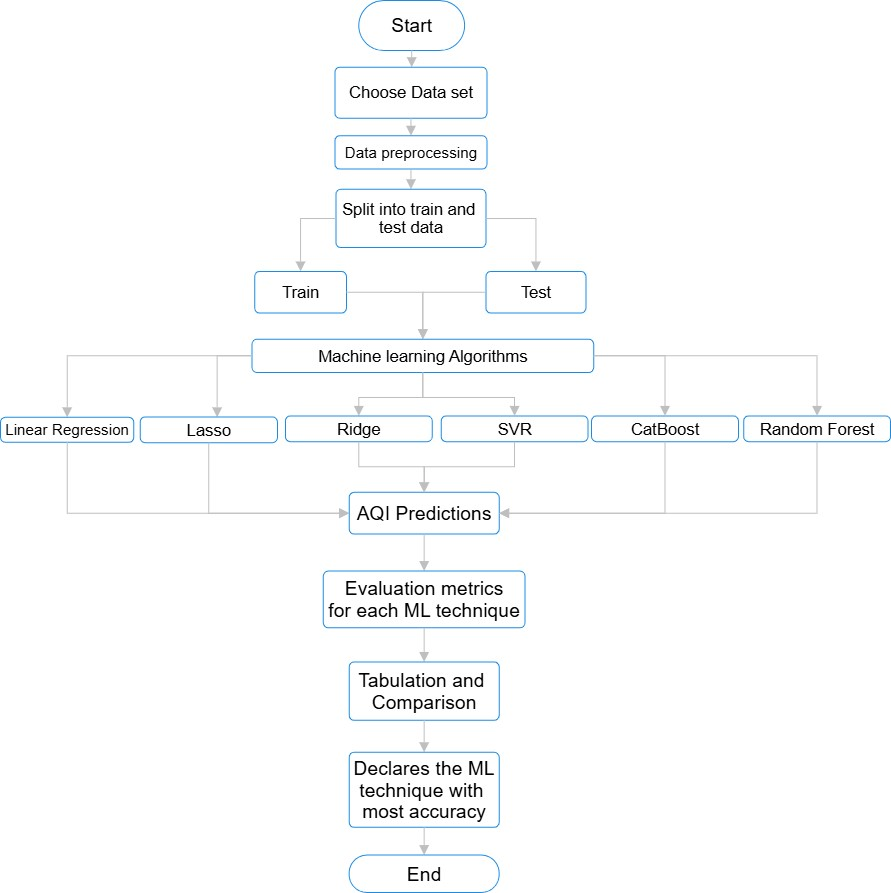
\includegraphics[width=0.8\linewidth]{flowchart.jpg}
    \caption{ Flow chart description of methodology}
    \label{fig:flowchart}
\end{figure}
%%-----------------------
\section{Data collection}
\label{data}
\vspace{-5mm} % Adjust the value to control the spacing
% Data was collected from Breathe Accra official website ({https://breatheaccra.org/}). 
Data was collected from Breathe Accra official website\footnote{https://breatheaccra.org/}{link to data at breathe Accra official website}).
The dataset contains air quality data and AQI of various areas in Accra the capital city of Ghana, these areas are; Dansoman, Kanda, Kawukudi, Korle-bu, and Kwashieman. dataset on each of these major areas in Accra were analyzed. The file size was 59.2MB with about 25898 rows and 30 columns. The variables contained in the dataset are; event, device, location, time, best latitude, best longitude, AQI, AQI level, Carbon monoxide, Carbon dioxide, humidity, Particulate Matter 1, Particulate Matter 2.5, Particulate Matter 10, pressure, temperature and voltage. The columns for pressure and humidity were empty so they were removed from the sample table. The samples of areas of Accra datasets are shown below.
 \begin{table}[H]
    \centering
        \caption{ Sample of the Dansoman dataset}
        \label{tab:Dansoman}
    \large % Increase the font size to \large, \Large, or \LARGE as needed
    \resizebox{1.1\textwidth}{!}{ % Resize the table to 110% of the text width
    \begin{tabular}{|c|c|c|c|c|c|c|c|c|c|c|}
        \hline
        Area & Time & CO & CO$_2$ & Humidity & PM$_{2.5}$ & PM$_{10}$ & Temp & Volt & AQI & AQI Bucket \\
        \hline
        Dansoman & 11/16/2023 23:37 & 850 & 2 & - & 6.066 & 6.6 & 27.876 & 4.207 & 25 & Good \\
        Dansoman & 11/16/2023 21:07 & 4360 & 23 & - & 37.512 & 45.490 & 28.437 & 4.227 & 106 & Unhealthy-if-Sensitive \\
        Dansoman & 11/16/2023 20:37 & 2543 & 14 & - & 23.135 & 27.756 & 28.375 & 4.227 & 74 & Moderate \\
        Dansoman & 11/15/2023 05:37 & 12413 & 44 & - & 78.048 & 83.146 & 25.438 & 4.176 & 163 & Unhealthy \\
        Dansoman & 11/11/2023 17:07 & 764 & 5 & - & 6.115 & 7.385 & 32.5 & 4.230 & 25 & Good \\
        \hline
    \end{tabular}
    }
    % \begin{tablenotes}
    %    % \item Sample of the Dansoman dataset.
    % \end{tablenotes}
\end{table}
\begin{table}[H]
    \centering
        \caption{Sample of Kwashieman cluster of schools dataset.}
        \label{tab:Kwashieman}
    \large
    \resizebox{1.1\textwidth}{!}{  
    \label{tab:kwashieman}
        \begin{tabular}{|c|c|c|c|c|c|c|c|c|c|c|} % Corrected column count to match headers
            \hline
            Area & Time & CO & CO$_2$ & Humidity & PM$_{2.5}$ & PM$_{10}$ & Temp & Volt & AQI & AQI Bucket \\
            \hline
            Kwashieman &11/16/2023 23:43 &1970 &5 &85.56577&14.885715 &16.314285 &27.617401 &4.1445312 &57 &moderate \\
            Kwashieman &11/16/2023 22:13&993 &- &82.79853 &4.806452 &4.806452 & 27.82779&4.15625 &20 &good \\
            Kwashieman &11/16/2023 16:43 &4750 &18 &63.68114 &36.425926 &43.148148 &30.133833 &4.1757812 &103&unhealthy-if-sensitive \\
            Kwashieman&11/16/2023 6:13 &10306 &56 &98.08832 &59.30612 &71.38776 &26.132326 &4.140625 & 153&unhealthy \\
            Kwashieman&11/15/2023 22:13 &2548 &5 & 90.88775&20.204546 &21.022728 &27.029041 &4.1601562 &68 &moderate \\
            \hline
        \end{tabular}
        }
        % \begin{tablenotes}
        %     \item Sample of Kwashieman cluster of schools dataset.
        % \end{tablenotes}
\end{table}
\begin{table}[H]
    \centering
        \caption{Sample of Kanda cluster of schools dataset}
        \label{tab:Kanda}
    \large
    \resizebox{1.1\textwidth}{!}{  
    \label{tab:kanda}
        \begin{tabular}{|c|c|c|c|c|c|c|c|c|c|c|} % Corrected column count to match headers
            \hline
            Area & Time & CO & CO$_2$ & Humidity & PM$_{2.5}$ & PM$_{10}$ & Temp & Volt & AQI & AQI Bucket \\
            \hline
            Kanda &11/16/2023 23:38 &684 &1 &85.5457&3.24 &3.24 &29.14886 &4.21875 &13 &good \\
            Kanda &11/16/2023 20:07&3487 &18 &77.815445 &30.846153 &34.05128 & 29.793074&4.234375 &90 &moderate \\
            Kanda &11/16/2023 16:43 &5085&19 &100 &38.239132 &45.760868 &27.817503 &4.1914062 &108&unhealthy-if-sensitive \\
            Kanda &11/12/2023 7:07&9076 &46 &100 &57.653847 &69.57692 &26.71981 &4.203125 & 152&unhealthy \\
            Kanda &11/12/2023 5:08 &2824 &7 & 100&23.324324 &24.378378 &26.191166 &4.2109375 &75 &moderate \\
            \hline
        \end{tabular}
        }
        % \begin{tablenotes}
        %     \item Sample of Kanda cluster of schools dataset.
        % \end{tablenotes}
\end{table}
\begin{table}[H]
    \centering
        \caption{Sample of Kawukudi cluster of schools dataset}
        \label{tab:Kawukudi}
    \large
    \resizebox{1.1\textwidth}{!}{  
    \label{tab:kawukudi}
        \begin{tabular}{|c|c|c|c|c|c|c|c|c|c|c|} % Corrected column count to match headers
            \hline
            Area & Time & CO & CO$_2$ & Humidity & PM$_{2.5}$ & PM$_{10}$ & Temp & Volt & AQI & AQI Bucket \\
            \hline
            Kawukudi &11/16/2023 23:41&3697 &14 &94.789085&29.860466 &32.34884 &27.248255 &4.2226562 &88 &moderate \\
            Kawukudi &11/16/2023 23:11&5367 &34 &93.210396&43.272728 &53.43182 & 27.424377&4.2265625 &120 &unhealthy-if-sensitive\\
            Kawukudi &11/16/2023 21:41&605 &8 &89.97582 &4.214286 &5.6666665 &27.76043 &4.2304688 &18&good \\
            Kawukudi&11/16/2023 16:41 &3449 &8 &65.36683 &25.59091 &28.568182 &31.555271 &4.140625 & 79&moderate \\
            Kawukudi &11/16/2023 6:41&9258 &61 & 100&62.980392 &74.45098 &25.93038 &4.1523438 &155 &unhealthy\\
            \hline
        \end{tabular}
        }
        % \begin{tablenotes}
        %     \item Sample of Kawukudi cluster of schools dataset.
        % \end{tablenotes}
\end{table}
\begin{table}[H]
    \centering
        \caption{Sample of Korle Bu cluster of schools dataset.}
        \label{tab:Korle Bu}
    \large
    \resizebox{1.1\textwidth}{!}{  
    \label{tab:korle bu}
        \begin{tabular}{|c|c|c|c|c|c|c|c|c|c|c|} % Corrected column count to match headers
            \hline
            Area & Time & CO & CO$_2$ & Humidity & PM$_{2.5}$ & PM$_{10}$ & Temp & Volt & AQI & AQI Bucket \\
            \hline
            Korle Bu &11/16/2023 23:50 &1030 &4&91.15001&6.892857 &8.464286 &28.01072 &3.9042969 &28 &good \\
            Korle Bu &11/16/2023 22:50&2376 &6 &90.2804 &18.38889 &19.972221 & 28.182102&3.90625 &64 &moderate \\
            Korle Bu &11/16/2023 9:50 &5676 &23 &70.90193 &39.745453 &49.109093 &33.51812 &3.9101562 &112&unhealthy-if-sensitive \\
            Korle Bu&11/16/2023 6:50 &13772 &49 &100 &72.85185 &80.75926 &27.260918 &3.9023438 & 160&unhealthy \\
            Korle Bu&11/16/2023 0:50&3399 &14 & 98.18342&29.177778 &33.066666 &27.534824 &3.9199219 &87 &moderate \\
            \hline
        \end{tabular}
        }
        % \begin{tablenotes}
        %     \item Sample of Korle Bu cluster of schools dataset.
        % \end{tablenotes}
\end{table}
%%%-------------------------------------
\section{Environment}
\label{environment}
To implement experimentation we used the following technologies. A brief description
of used technologies is represented below:
\begin{itemize}
\item Python - Python is an interpreted, high-level, object-oriented programming language. It is an open source.
\item Anaconda navigator - It is a graphical user interface (GUI) that allows to launch applications easily and manage packages.
\item Jupyter notebook - It is a web-based interactive computing platform. It helps in developing, documenting, and executing code.
\item Pandas- It is an open-source Python library that is freely available. Primarily, it is utilized for data analysis and facilitates a range of data manipulation tasks.
\item Numpy- It is a Python library designed for scientific computing, enabling a broad range of mathematical operations on data.
\item Matplotlib- It is a Python package for creating static, animated, and interactive visualizations.
\item Seaborn- It is a Python library for data visualization, built on top of the matplotlib library. It facilitates the creation of statistical graphics using Python.
\item Scikit-learn (sklearn) - It is a Python library for machine learning, predominantly written in Python. It includes a variety of machine learning algorithms and is particularly well-suited for predictive analysis.
\end{itemize}
\section{Data preprocessing}
\label{preprocessing}
Data preprocessing is a critical step in the data analysis process. It involves preparing and transforming raw data into a clean and usable format. For an AQI dataset, preprocessing typically includes several steps: data cleaning, handling missing values, normalizing or scaling data, encoding categorical variables, and feature selection.
%---------------------------
\subsection{Data cleaning}
\label{cleaning}
Data cleaning involves identifying and correcting errors or inconsistencies in the dataset to ensure the data is accurate and consistent.
\begin{enumerate}
\item Removing duplicates: Check for and remove any duplicate rows in the dataset.
\item Correcting inconsistencies: Ensure consistency in data formats
\end{enumerate}
%------------------------------
\subsection{Handling Missing Values}
\label{handling}
Missing values can significantly impact the analysis. Common methods to handle missing values include deleting entire rows with missing values or inputting the missing values. But when challenged with very large data and one opts to input missing values, the authenticity of the dataset may be compromised. For smaller datasets or when missing data is minimal, inputting missing values using mean, median or mode is a good practice. For our case, rows with missing values were removed.
%%-------------------
\subsection{Normalizing or Scaling Data}
\label{normalizing}
Normalizing or scaling ensures that all numerical features are on the same scale, which is particularly important for algorithms that compute distances between data points like K-nearest neighbors, and SVM.
%%--------------------
\subsection{Feature Selection}
\label{feature}
Feature selection involves selecting the most important features that contribute to the prediction variable or output. This helps in improving model performance and reducing overfitting. Particulate matter 2.5 and 10  were our features to predict the  AQI value.\\
\begin{itemize}
\vspace{-5mm} % Adjust the value to control the spacing
\item Correlation Matrix: check the correlation between features and select those with high correlation to the target variable. PM$_{2.5}$ and PM$_{10}$ were highly correlated with the target variable and the correlation between them was negligible. 
\end{itemize}
%------------------------------
\section{Training and testing the model}
\vspace{-10pt} % Adjust space after section title
\label{training}
Firstly, we collected the dataset from the Breathe Accra site. Then the preprocessing techniques like data cleaning, handling missing values, normalization, and feature selection on the data were executed. At first, the data related to the particular area in Accra is extracted. After that, all the tuples which have missing values were ignored. Further data cleaning is performed for better and more accurate results. Then data is split into two parameters which contain air particle composition in one parameter and AQI data in another parameter. PM\textsubscript{2.5} and PM\textsubscript{10} variables were considered for predicting the AQI variable. We divided the data into 70 percent training data and 30 percent testing data. Matplotlib library was used to visualize how well the predicted values match the actual values using scatter plot graphs and line plots. The machine learning algorithms that were identified from the literature review such as linear regression, LASSO regression, ridge regression, SVR algorithm, Random forest, and CatBoost were used to build prediction models. The same data that was preprocessed were used to train the model with all the identified algorithms. At first, a model is built using a linear regression algorithm followed by LASSO regression, ridge regression, SVR, random forest, and catBoost. Building a machine learning model involves analyzing data to identify patterns and make predictions. Then the built models will be tested by calculating the performance metrics. These performance metrics will test how well the model can predict the AQI.
\section{Performance metrics}
\label{performance}
In the realm of air quality, the selection and application of appropriate evaluation metrics are paramount to accurately assess and interpret the performance of predictive models. These metrics provide quantitative measures that reflect the model's ability to generalize to new data, capture relevant patterns, and make reliable predictions. Different types of metrics cater to different aspects of model performance. This section delves into various commonly used evaluation metrics, explaining their significance and the context in which they are most useful.
In regression analysis, metrics like Mean Absolute Error (MAE), Mean Squared Error (MSE), Root Mean Squared Error (RMSE), R-squared, and Adjusted R-squared are used to quantify the discrepancies between predicted and actual values. These metrics provide insights into the model's accuracy and its ability to generalize to unseen data. They are particularly useful in continuous prediction scenarios, such as forecasting pollutant concentrations. The subsequent sections will provide a detailed explanation of each metric, outlining their formulas, components, and importance in the context of air quality research.
\vspace{-5mm} % Adjust the value to control the spacing
\subsection{Mean Absolute Error (MAE)}
\label{mae}
\vspace{-5mm} % Adjust the value to control the spacing
The average of the absolute differences between predicted and actual values. Provides a direct measure of the average magnitude of errors without considering their direction. Useful when all errors are equally important\cite{MAE_ref}.\\
$$\text{MAE} = \frac{1}{N} \sum_{i=1}^{N} |y_i - \hat{y}_i|,$$
where\\
 N: The number of observations.\\
$y_i$: The actual value for the ${i-th}$ observation.\\
$\hat{y}_i$: The predicted value for the ${i-th}$ observation.
%-------------------------------------------------
\vspace{-5mm} % Adjust the value to control the spacing
\subsection{Root Mean Squared Error (RMSE)}
\label{rmse}
\vspace{-5mm} % Adjust the value to control the spacing
It is the square root of the mean squared error. It also provides an error measure in the same units as the target variable, making interpretation easier\cite{RMSE_ref}.\\
$$\text{RMSE} = \sqrt{\frac{1}{N} \sum_{i=1}^{N} (y_i - \hat{y}_i)^2},$$
where\\
 N: The number of observations.\\
 $y_i$: The actual value for the $i{-th}$ observation.\\
$\hat{y}_i$ : The predicted value for the ${i-th}$ observation.

\vspace{-5mm} % Adjust the value to control the spacing
\subsection{R-squared (Coefficient of Determination)}
\label{r}
\vspace{-5mm} % Adjust the value to control the spacing
It indicates the proportion of variance in the dependent variable that is predictable from the independent variables. Provides an overall measure of how well the model explains the observed outcomes. A higher value indicates a better fit\cite{R2_ref}.\\
$$R^2 = 1 - \frac{\sum_{i=1}^{N} (y_i - \hat{y}_i)^2}{\sum_{i=1}^{N} (y_i - \bar{y})^2},$$
where\\
 N: The number of observations.\\
 $y_i$: The actual value for the ${i-th}$ observation.\\
$\hat{y}_i$ : The predicted value for the ${i-th}$ observation.\\ 
$\bar{y}$ : The mean of the actual values.

\vspace{-5mm} % Adjust the value to control the spacing
\subsection{Importance of Performance metrics}
\label{importance}
\vspace{-5mm} % Adjust the value to control the spacing
\begin{enumerate}
    \item Model Selection: Metrics help in selecting the best model among multiple candidates by providing quantitative measures of performance.
    \item Performance Evaluation: Metrics allow for the objective evaluation of a model’s performance, indicating areas for improvement.
    \item Hyperparameter Tuning: Metrics guide the tuning of hyperparameters to optimize model performance.
    \item Comparing Models: Metrics provide a standardized way to compare different models and algorithms.
\end{enumerate}
%%%-------------------------------------------
\chapter{Numerical Results}
\label{ch4}
\vspace{-5mm} % Adjust the value to control the spacing
\section{Experimentation outcome}
\label{experimentation}
\vspace{-5mm} % Adjust the value to control the spacing
This section shows the analysis of the experiment with the preprocessed dataset of each area in Accra and the identified machine learning algorithms from the literature review. For the same collection of air quality data, Linear regression, LASSO regression, Ridge regression, SVR, Random forest and CatBoost  are used to build the model individually. For experimentation purposes, feature variables were PM 2.5 and PM 10 attributes as our input to obtain the AQI attribute which is the final output. The various areas will be taken one after the other for analysis.
\vspace{-5mm} % Adjust the value to control the spacing
\section{Dansoman}
\label{dansoman}
\vspace{-5mm} % Adjust the value to control the spacing
\subsection{Linear Regression}
\vspace{-5mm} % Adjust the value to control the spacing
The data is preprocessed and trained with a linear regression algorithm to predict the AQI.
%%%----------------------------------
\vspace{-5mm} % Adjust the value to control the spacing
\begin{table}[H]
    \centering
    \begin{tabular}{|c|c|}
        \hline
        \textbf{Metric} & \textbf{Value} \\
        \hline
        MAE & 6.3633 \\
        \hline
        RMSE & 8.6067 \\
        \hline
        R-square & 0.9455 \\
        \hline
    \end{tabular}
    \caption{Metrics for Linear Regression (Dansoman)}
    \label{tab: Linear metrics(Dansoman)}
\end{table}
%------------------------------
The figure is a scatter plot graph. Here, the X-axis and Y-axis are the observed AQI value and predicted AQI value, respectively.
%-----------------------------
\vspace{-5mm} % Adjust the value to control the spacing
\begin{figure}[H]
    \centering
    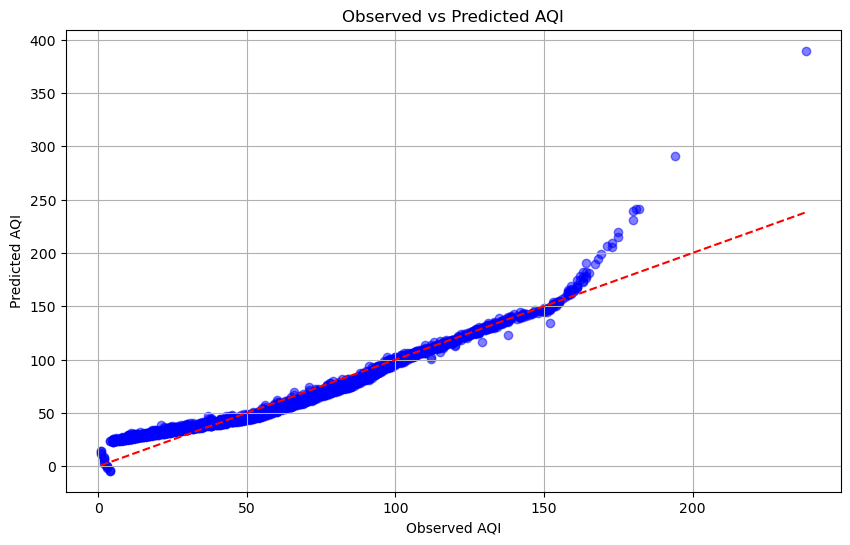
\includegraphics[width=\linewidth]{dansoman scatter plot.png}
    \caption{ Scatter plot Linear Regression (Dansoman)}
    \label{fig: Linear scatter plot(Dansoman)}
\end{figure}
%-------------------------------
The figure is a graph that shows how predicted values using the linear regression algorithm on the Dansoman dataset were similar to observed values. Here the X-axis and Y-axis are Time and AQI values respectively.
\begin{figure}[H]
    \centering
        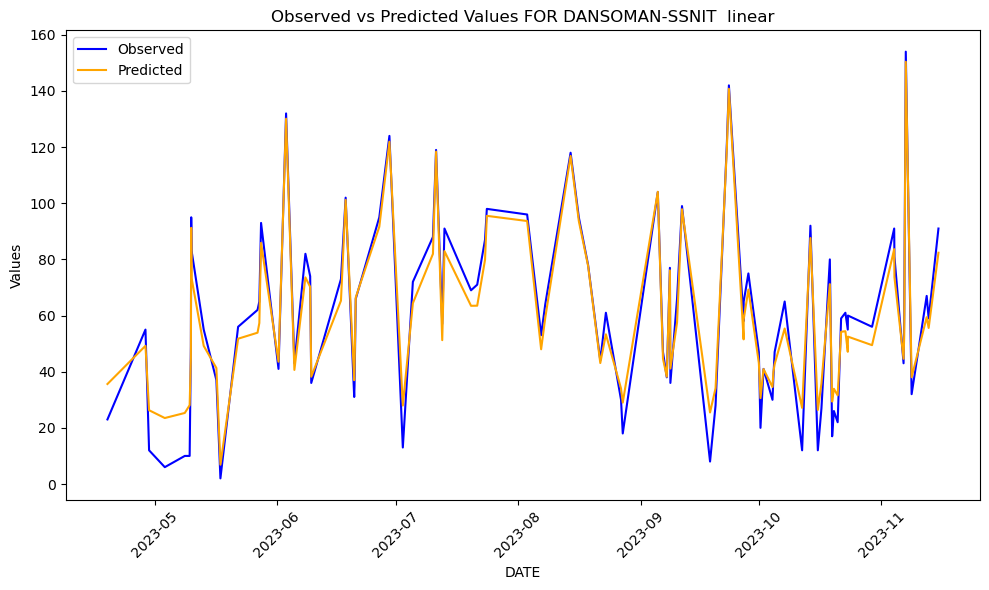
\includegraphics[width=\linewidth]{dansoman linear plot.png}
        \caption{ Predicted vs observed AQI Linear regression (Dansoman)}
         \label{fig: Linear Predicted vs observed(Dansoman)}
\end{figure}
\vspace{-5mm} % Adjust the value to control the spacing
 \subsection{LASSO Regression}
 \vspace{-5mm} % Adjust the value to control the spacing
The data is preprocessed and trained with the LASSO regression algorithm to predict the AQI. The performance matrix is illustrated in the table below.
%%%----------------------------------
\begin{table}[H]
    \centering
    \begin{tabular}{|c|c|}
        \hline
        \textbf{Metric} & \textbf{Value} \\
        \hline
        MAE & 6.4828 \\
        \hline
        RMSE & 9.6909 \\
        \hline
        R-square & 0.9311 \\
        \hline
    \end{tabular}
    \caption{Metrics for the LASSO Regression (Dansoman)}
    \label{tab: LASSO metrics (Dansoman)}
\end{table}
\begin{figure}[H]
 \begin{minipage}{\linewidth}
        The figure is a graph that shows how predicted values using the LASSO regression algorithm on the Dansoman dataset were similar to observed values. Here the X-axis and Y-axis are Time and AQI values respectively.
        \vspace{0.5em} 
        \includegraphics[width=\linewidth]{LASSO line plot.png}
       \caption{ Predicted vs observed AQI values LASSO (Dansoman)}
        \label{fig: LASSO Predicted vs observed AQI(Dansoman)}
    \end{minipage}
\end{figure}
\vspace{-5mm} % Adjust the value to control the spacing
\subsection{Ridge}
\vspace{-5mm} % Adjust the value to control the spacing
The data is preprocessed and trained with a Ridge regression algorithm to predict the AQI.
%%%----------------------------------
\begin{table}[H]
    \centering
    \begin{tabular}{|c|c|}
        \hline
        \textbf{Metric} & \textbf{Value} \\
        \hline
        MAE & 6.4812 \\
        \hline
        RMSE & 9.6909\\
        \hline
        R-square & 0.9311 \\
        \hline
    \end{tabular}
    \caption{Metrics for Ridge Regression (Dansoman)}
    \label{tab: Ridge metrics(Dansoman)}
\end{table}
%%-----------------------------
The figure below is a graph that shows how predicted values using the Ridge regression algorithm on the Dansoman dataset were similar to observed values. Here the X-axis and Y-axis are Time and AQI values respectively.
%%----------------------------------
\begin{figure}[H]
\centering 
       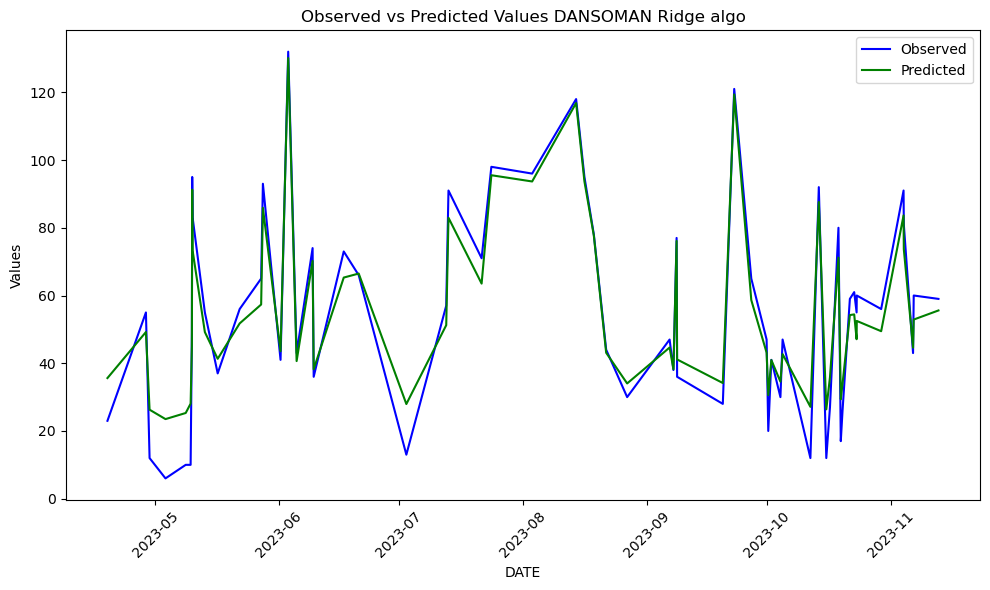
\includegraphics[width=\linewidth]{ridge dansoman.png}
        \caption{ Predicted vs observed AQI Ridge(Dansoman)}
        \label{fig: Ridge predicted vs observed AQI(Dansoman)}
\end{figure}
\subsection{Support Vector Regression}
The data is preprocessed and trained with a Support Vector Regression algorithm to predict the AQI. The table below shows the performance of the support vector regression after being implemented.
%%----------------------------------
\begin{table}[H]
    \centering
    \begin{tabular}{|c|c|}
        \hline
        \textbf{Metric} & \textbf{Value} \\
        \hline
        MAE & 0.7714 \\
        \hline
        RMSE & 2.9456\\
        \hline
        R-square & 0.9936 \\
        \hline
    \end{tabular}
    \caption{ Metrics for Support Vector Regression (Dansoman)}
    \label{tab:SVR metrics(Dansoman)}
\end{table}
%%-----------------------
The figure below is a graph that shows how predicted values using the Support Vector Regression algorithm on the Dansoman dataset were very similar to observed values. Here the X-axis and Y-axis are Time and AQI values respectively.
%%=-------------------------
\begin{figure}[H]
 \centering
        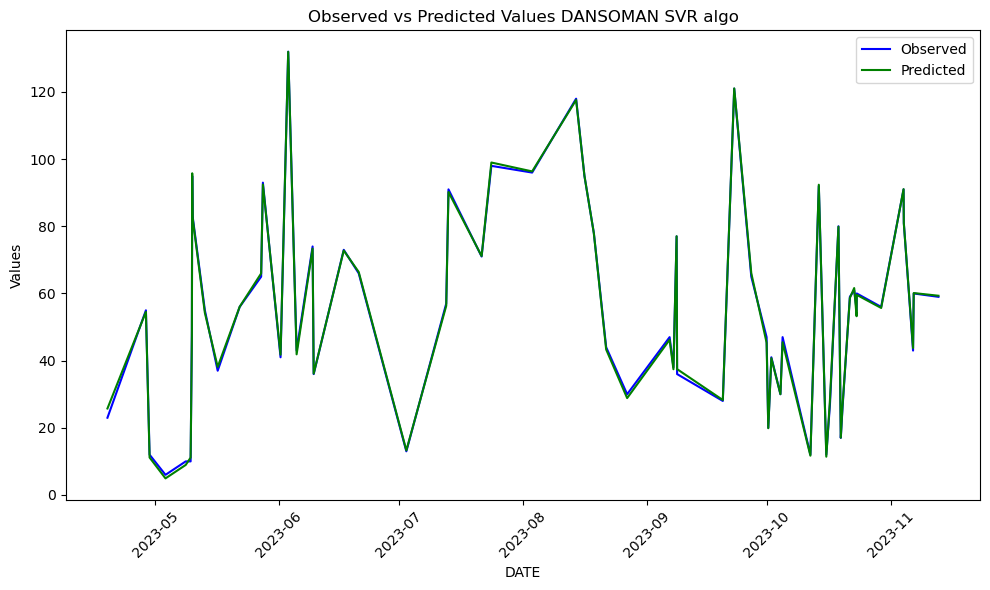
\includegraphics[width=\linewidth]{SVR line graph.png}
        \caption{ Predicted vs observed AQI SVR (Dansoman)}
        \label{fig: SVR predicted vs observed AQI(Dansoman)}
\end{figure}
%--------------------------------
\subsection{Random Forest Regression} 
The data is preprocessed and trained with the random forest regression algorithm to predict the AQI.
\begin{table}[H]
    \centering
    \begin{tabular}{|c|c|}
        \hline
        \textbf{Metric} & \textbf{Value} \\
        \hline
        MAE & 0.0262 \\
        \hline
        RMSE & 0.1185\\
        \hline
        R-square & 1.0000 \\
        \hline
    \end{tabular}
    \caption{Metrics for Random Forest  (Dansoman)}
    \label{tab: RFR metrics(Dansoman)}
\end{table}
%%--------------------------
The figure below is a graph that shows how predicted values using the Random Forest Regression algorithm on the Dansoman dataset were very similar to observed values. Here the X-axis and Y-axis are Time and AQI values respectively.
%0----------------------------
\begin{figure}[H]
 \centering
        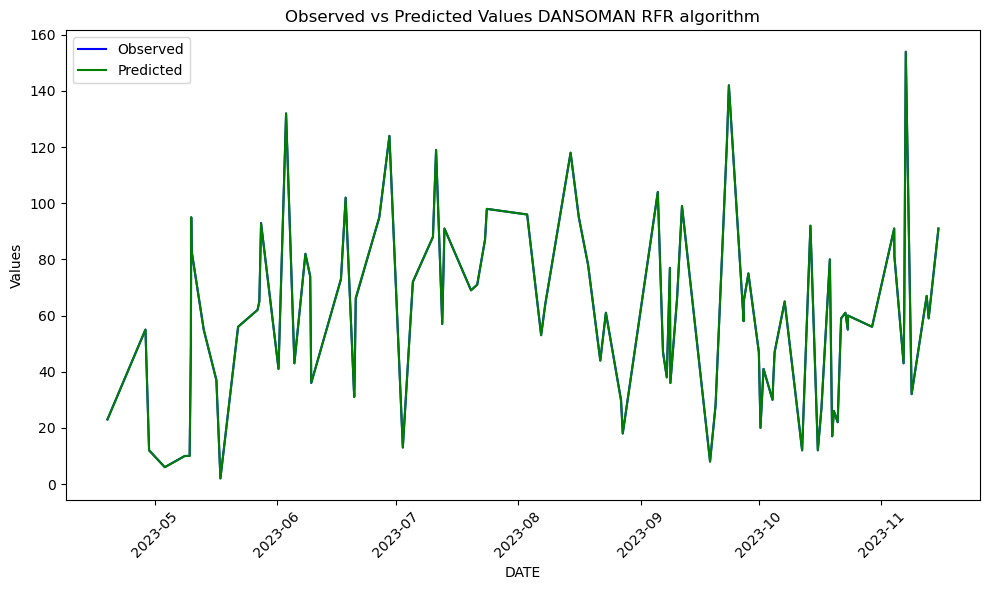
\includegraphics[width=\linewidth]{RFR line plot.png}
        \caption{ Predicted vs observed AQI values RFR (Dansoman)}
        \label{fig: RFR Predicted vs observed AQI(Dansoman)}
\end{figure}
\subsection{CatBoost Regression} 
The data is preprocessed and trained with the CatBoost Regression algorithm to predict the AQI.
\begin{table}[H]
    \centering
    \begin{tabular}{|c|c|}
        \hline
        \textbf{Metric} & \textbf{Value} \\
        \hline
        MAE & 0.2947 \\
        \hline
        RMSE & 0.7402\\
        \hline
        R-square & 1.0000 \\
        \hline
    \end{tabular}
    
    \caption{Metrics for the Catboost Regression (Dansoman)}
    \label{tab: CBR metrics(Dansoman)}
\end{table}
%%%----------------------------
The figure below is a graph that shows how predicted values using the Catboost Regression algorithm on the Dansoman dataset were very similar to observed values. Here the X-axis and Y-axis are Time and AQI values respectively.
%%-------------------
\begin{figure}[H]
 \centering
        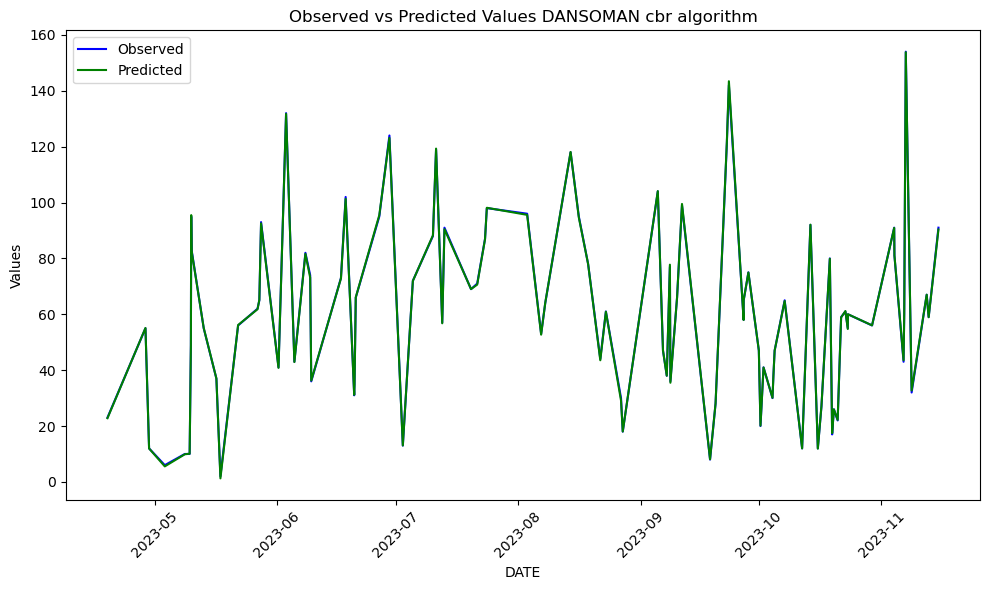
\includegraphics[width=\linewidth]{dansoman cbr.png}
       
        \caption{ Predicted vs observed AQI Catboost(Dansoman)}
        \label{fig: CBR Predicted vs observed AQI(Dansoman)}
\end{figure}   
%%--------------------------

\section{Kanda}
\label{kanda}
\subsection{Linear Regression}
The data is preprocessed and trained with the linear regression algorithm to predict the AQI. The table below shows the performance metrics after the algorithm was tested.
\begin{table}[H]
    \centering
    \begin{tabular}{|c|c|}
        \hline
        \textbf{Metric} & \textbf{Value} \\
        \hline
        MAE & 4.8870 \\
        \hline
        RMSE & 8.1989 \\
        \hline
        R-square & 0.9435 \\
        \hline
    \end{tabular}
    \caption{Metrics for Linear Regression (Kanda)}
    \label{tab: Linear metrics(Kanda)}
\end{table}
\begin{figure}[H]
 \begin{minipage}{\linewidth}
        The figure below is a graph that shows how predicted values using the linear Regression algorithm on the Kanda dataset were similar to observed values. Here the X-axis and Y-axis are Time and AQI values respectively.
        \vspace{0.5em} 
        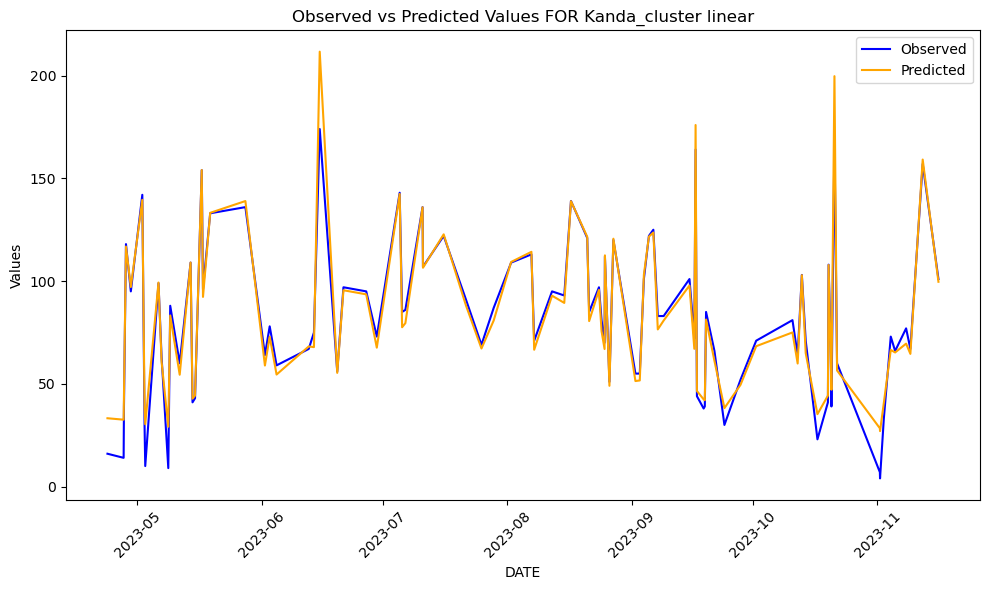
\includegraphics[width=\linewidth]{kanda linear.png}
       
        \caption{ Predicted vs observed AQI Linear regression (Kanda)}
        \label{fig: Linear Predicted vs observed AQI(Kanda)}
    \end{minipage}
\end{figure}
\subsection{LASSO}
The data is preprocessed and trained with the LASSO regression algorithm to predict the AQI. The table below shows the performance metrics after the LASSO regression model was configured on the Kanda dataset.\\
\begin{table}[H]
    \centering
    \begin{tabular}{|c|c|}
        \hline
        \textbf{Metric} & \textbf{Value} \\
        \hline
        MAE & 4.9546 \\
        \hline
        RMSE & 8.1768 \\
        \hline
        R-square & 0.9457 \\
        \hline
    \end{tabular}
    \caption{Metrics for LASSO Regression (Kanda)}
    \label{tab: LASSO metrics(Kanda)}
\end{table}
\begin{figure}[H]
 \begin{minipage}{\linewidth}
        The figure below is a graph that shows how predicted values using the LASSO Regression algorithm on the Kanda dataset were similar to observed values. Here the X-axis and Y-axis are Time and AQI values respectively.
        \vspace{0.5em} 
        \includegraphics[width=\linewidth]{kanda LASSO.png}
       
        \caption{ Predicted vs observed AQI LASSO(Kanda)}
        \label{fig: LASSO Predicted vs observed AQI(Kanda)}
    \end{minipage}
\end{figure}
\subsection{Ridge Regression}
The data is preprocessed and trained with the Ridge regression algorithm to predict the AQI. The table below shows the performance metrics after the model configuration on the Kanda dataset.\\
\begin{table}[H]
    \centering
    \begin{tabular}{|c|c|}
        \hline
        \textbf{Metric} & \textbf{Value} \\
        \hline
        MAE & 4.9538 \\
        \hline
        RMSE & 8.1768 \\
        \hline
        R-square & 0.9457 \\
        \hline
    \end{tabular}
    \caption{Metrics for Ridge Regression (Kanda)}
    \label{tab: Ridge metrics(Kanda)}
\end{table}
\begin{figure}[H]
 \begin{minipage}{\linewidth}
        The figure below is a graph that shows how predicted values using Ridge Regression algorithm on Kanda dataset were similar to observed values. Here the X-axis and Y-axis are Time and AQI value respectively.
        \vspace{0.5em} 
        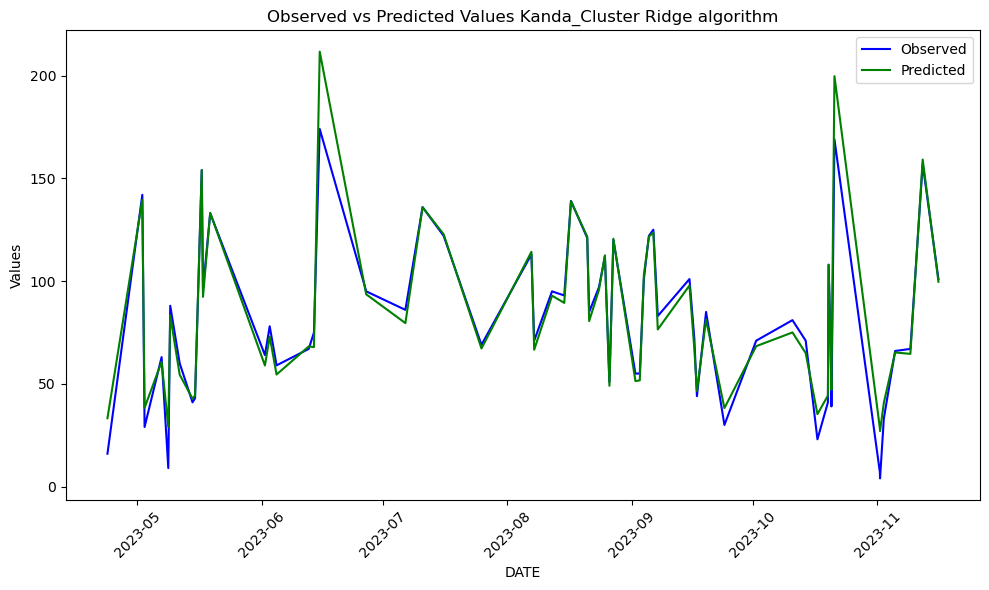
\includegraphics[width=\linewidth]{Kanda Ridge.png}
       
        \caption{ Predicted vs observed AQI Ridge regression (Kanda)}
        \label{fig: Ridge predicted vs observed AQI(Kanda)}
    \end{minipage}
\end{figure}
\subsection{Support Vector Regression}
The data is preprocessed and trained with a Support Vector Regression algorithm to predict the AQI. The table below shows the performance metrics after the model configuration on the Kanda dataset.\\
\begin{table}[H]
    \centering
    \begin{tabular}{|c|c|}
        \hline
        \textbf{Metric} & \textbf{Value} \\
        \hline
        MAE & 0.7681 \\
        \hline
        RMSE & 4.7741 \\
        \hline
        R-square & 0.809 \\
        \hline
    \end{tabular}
    \caption{Metrics for Support Vector Regression (Kanda) }
    \label{tab: SVR metrics(Kanda)}
\end{table}
\begin{figure}[H]
 \begin{minipage}{\linewidth}
        The figure below is a graph that shows how predicted values using the Ridge Regression algorithm on Kanda dataset were similar to observed values. Here the X-axis and Y-axis are Time and AQI values respectively.
        \vspace{0.5em} 
        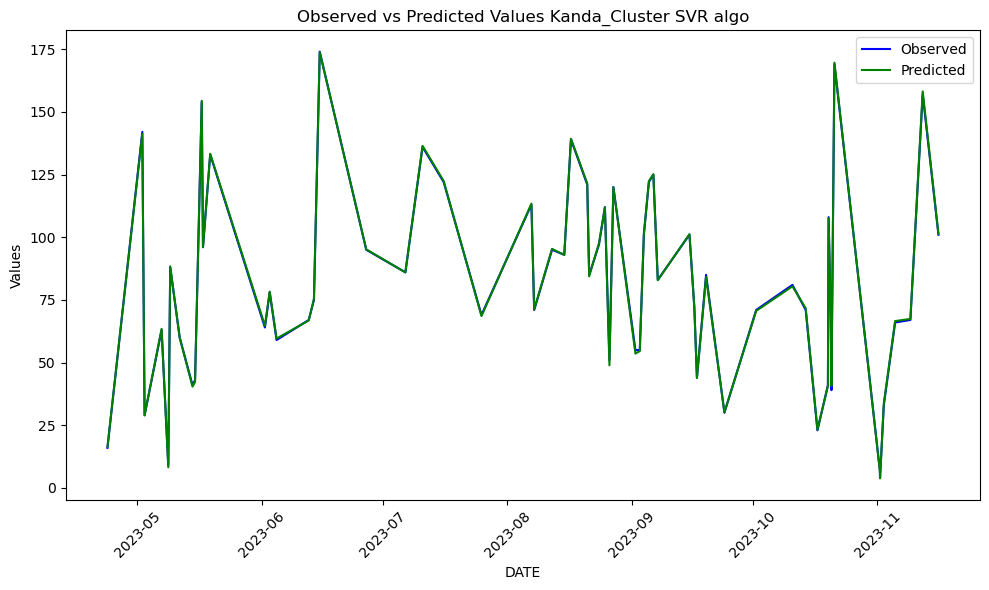
\includegraphics[width=\linewidth]{kand svr.png}
       
        \caption{ predicted vs observed AQI SVR (Kanda)}
        \label{fig: SVR predicted vs observed AQI(Kanda)}
    \end{minipage}
\end{figure}
\subsection{Random Forest Regression}
The data is preprocessed and trained with the random forest regression algorithm to predict the AQI. The table below shows the performance metrics after the model was configured on the Kanda dataset.\\
\begin{table}[H]
    \centering
    \begin{tabular}{|c|c|}
        \hline
        \textbf{Metric} & \textbf{Value} \\
        \hline
        MAE & 0.03361 \\
        \hline
        RMSE & 0.2948 \\
        \hline
        R-square & 0.9999\\
        \hline
    \end{tabular}
    \caption{Metrics for Random Forest Regression (Kanda)}
    \label{tab: RFR metrics(Kanda)}
\end{table}
\begin{figure}[H]
 \begin{minipage}{\linewidth}
        The figure below is a graph that shows how predicted values using the Random Forest Regression algorithm on Kanda dataset were similar to observed values. Here the X-axis and Y-axis are Time and AQI values respectively.
        \vspace{0.5em} 
        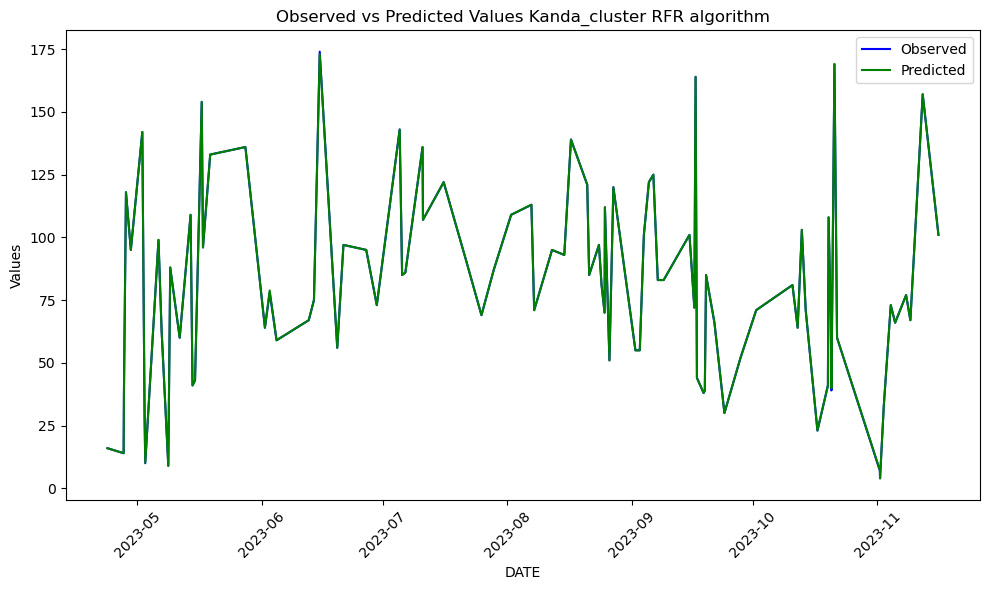
\includegraphics[width=\linewidth]{kand rfr.png}
       
        \caption{ Predicted vs observed AQI RFR (Kanda)}
        \label{fig: RFR predicted vs observed AQI(Kanda)}
    \end{minipage}
\end{figure}
\subsection{CatBoost Regression}
The data is preprocessed and trained with CatBoost Regression algorithm to predict the AQI. The table below shows the performance metrics after the model was configured on the Kanda dataset.\\
\begin{table}[H]
    \centering
    \begin{tabular}{|c|c|}
        \hline
        \textbf{Metric} & \textbf{Value} \\
        \hline
        MAE & 0.3058 \\
        \hline
        RMSE & 1.0185 \\
        \hline
        R-square & 0.9991\\
        \hline
    \end{tabular}
    \caption{Metrics for the CatBoost Regression (Kanda)}
    \label{tab: CBR metrics(Kanda)}
\end{table}
\begin{figure}[H]
 \begin{minipage}{\linewidth}
        The figure below is a graph that shows how predicted values using the CatBoost Regression algorithm on Kanda dataset were similar to observed values. Here the X-axis and Y-axis are Time and AQI values respectively.
        \vspace{0.5em} 
        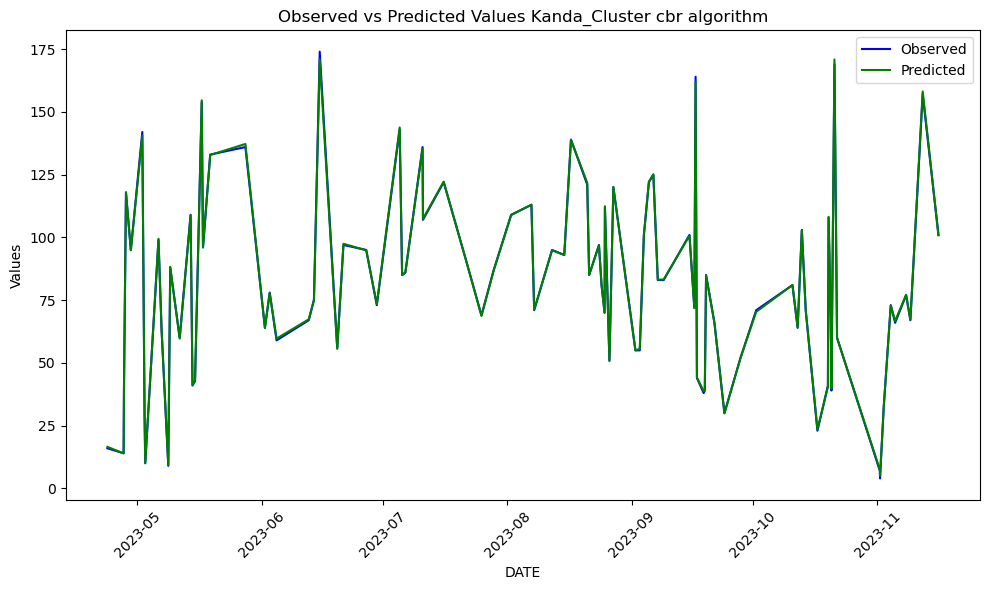
\includegraphics[width=\linewidth]{kanda cbr.png}
       
        \caption{ Predicted vs observed AQI CatBoost (Kanda)}
        \label{fig: CBR predicted vs observed AQI(Kanda)}
    \end{minipage}
\end{figure}

\vspace{-5mm} % Adjust the value to control the spacing
\section{Kawukudi}
\label{kawukudi}
\vspace{-5mm} % Adjust the value to control the spacing
\subsection{Linear Regression}
\vspace{-5mm} % Adjust the value to control the spacing
The data is preprocessed and trained with linear regression algorithm to predict the AQI. The table below shows the performance metrics after the algorithm was tested.\\
\begin{table}[H]
    \centering
    \begin{tabular}{|c|c|}
        \hline
        \textbf{Metric} & \textbf{Value} \\
        \hline
        MAE & 7.8628 \\
        \hline
        RMSE & 12.8249 \\
        \hline
        R-square & 0.8839 \\
        \hline
    \end{tabular}
    \caption{Metrics for Linear Regression (Kawukudi)}
    \label{tab: Linear metrics(Kawukudi)}
\end{table}
\begin{figure}[H]
 \begin{minipage}{\linewidth}
        The figure below is a graph which shows how predicted values using linear Regression algorithm on Kawukudi dataset were similar to observed values. Here the X-axis and Y-axis are Time and AQI value respectively.
        \vspace{0.5em} 
        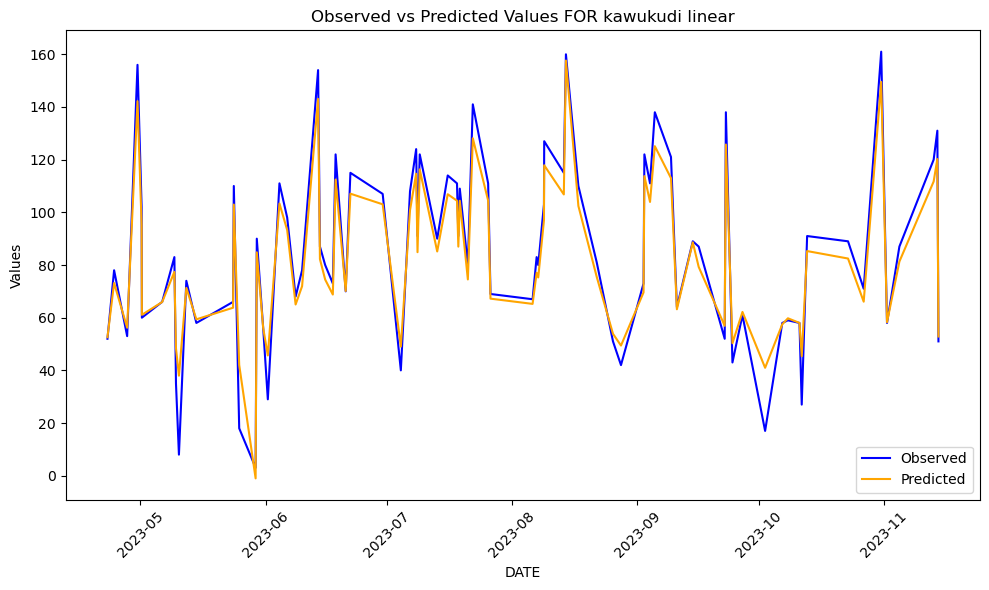
\includegraphics[width=\linewidth]{kawukudi linear.png}
       
        \caption{ Predicted vs observed AQI Linear regression (Kawukudi)}
        \label{fig: Linear predicted vs observed AQI(Kawukudi)}
    \end{minipage}
\end{figure}
\subsection{LASSO}
The data is preprocessed and trained with LASSO regression algorithm to predict the AQI. The table below shows the performance metrics after the LASSO regression model was configured on the Kawukudi dataset.\\
\begin{table}[H]
    \centering
    \begin{tabular}{|c|c|}
        \hline
        \textbf{Metric} & \textbf{Value} \\
        \hline
        MAE & 7.8263 \\
        \hline
        RMSE & 12.7065 \\
        \hline
        R-square & 0.8861 \\
        \hline
    \end{tabular}
    \caption{Metrics for LASSO Regression (Kawukudi)}
    \label{tab: LASSO metrics(Kawukudi)}
\end{table}
\begin{figure}[H]
 \begin{minipage}{\linewidth}
        The figure below is a graph that shows how predicted values using the LASSO Regression algorithm on the Kawukudi dataset were similar to observed values. Here the X-axis and Y-axis are Time and AQI values respectively.
        \vspace{0.5em} 
        \includegraphics[width=\linewidth]{kawukudi LASSO.png}
       
        \caption{ Predicted vs observed AQI LASSO regression (Kawukudi)}
        \label{fig: LASSO predicted vs observed AQI(Kawukudi)}
    \end{minipage}
\end{figure}
\subsection{Ridge Regression}
The data is preprocessed and trained with Ridge regression algorithm to predict the AQI. The table below shows the performance metrics after the model was configured on the Kawukudi dataset.\\
\begin{table}[H]
    \centering
    \begin{tabular}{|c|c|}
        \hline
        \textbf{Metric} & \textbf{Value} \\
        \hline
        MAE & 7.8249 \\
        \hline
        RMSE & 12.7065\\
        \hline
        R-square & 0.8861 \\
        \hline
    \end{tabular}
    \caption{Metrics for Ridge Regression (Kawukudi)}
    \label{tab: Ridge metrics(Kawukudi)}
\end{table}
\begin{figure}[H]
 \begin{minipage}{\linewidth}
        The figure below is a graph that shows how predicted values using the Ridge Regression algorithm on the Kawukudi dataset were similar to observed values. Here the X-axis and Y-axis are Time and AQI values respectively.
        \vspace{0.5em} 
        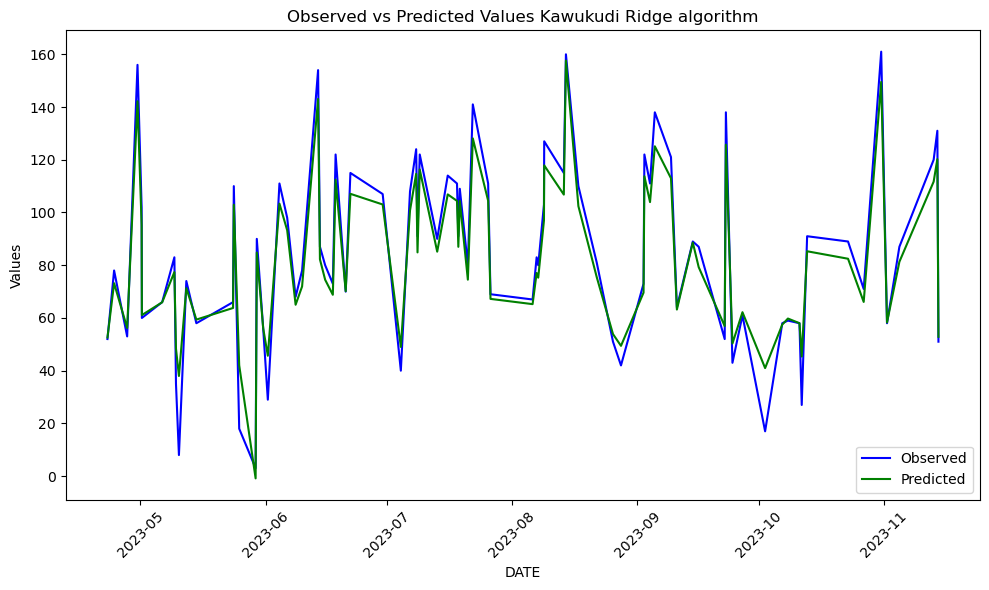
\includegraphics[width=\linewidth]{kawukudi ridge.png}
       
        \caption{ Predicted vs observed AQI Ridge regression (kawukudi)}
        \label{fig: Ridge predicted vs observed AQI(Kawukudi)}
    \end{minipage}
\end{figure}
\subsection{Support Vector Regression}
The data is preprocessed and trained with Support Vector Regression algorithm to predict the AQI. The table below shows the performance metrics after the model was configured on the Kawukudi dataset.\\
\begin{table}[H]
    \centering
    \begin{tabular}{|c|c|}
        \hline
        \textbf{Metric} & \textbf{Value} \\
        \hline
        MAE & 1.0098 \\
        \hline
        RMSE & 6.7301 \\
        \hline
        R-square & 0.9680 \\
        \hline
    \end{tabular}
    \caption{Metrics for Support Vector regression (kawukudi)}
    \label{tab: SVR metrics(Kawukudi)}
\end{table}
\begin{figure}[H]
 \begin{minipage}{\linewidth}
        The figure below is a graph that shows how predicted values using the Support Vector Regression algorithm on the Kawukudi dataset were similar to observed values. Here the X-axis and Y-axis are Time and AQI values respectively.
        \vspace{0.5em} 
        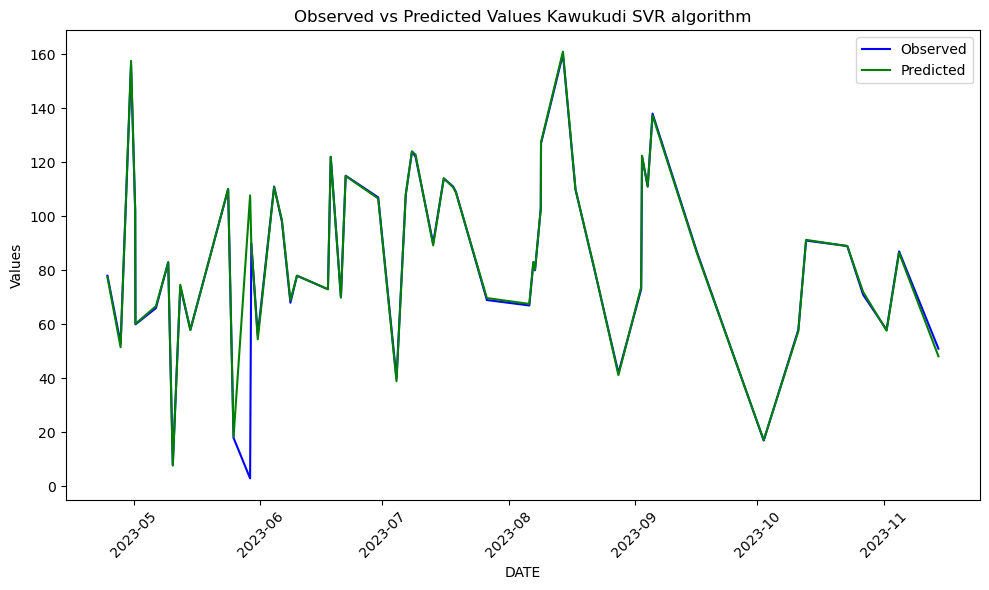
\includegraphics[width=\linewidth]{kawukudi svr.png}
       
        \caption{ Predicted vs observed AQI SVR (kawukudi)}
        \label{fig: SVR predicted vs observed AQI(Kawukudi)}
    \end{minipage}
\end{figure}
\subsection{Random Forest Regression}
The data is preprocessed and trained with the random forest regression algorithm to predict the AQI.\\ The table below shows the performance metrics after the model was configured on the Kawukudi dataset.\\
\begin{table}[H]
    \centering
    \begin{tabular}{|c|c|}
        \hline
        \textbf{Metric} & \textbf{Value} \\
        \hline
        MAE & 0.0415 \\
        \hline
        RMSE & 0.2702\\
        \hline
        R-square & 0.9999\\
        \hline
    \end{tabular}
    \caption{Metrics for Random Forest (Kawukudi)}
    \label{tab: RFR metrics(Kawukudi)}
\end{table}
\begin{figure}[H]
 \begin{minipage}{\linewidth}
        The figure below is a graph that shows how predicted values using the Random Forest Regression algorithm on the Kawukudi dataset were very similar to observed values. \\Here the X-axis and Y-axis are Time and AQI values respectively.
        \vspace{0.5em} 
        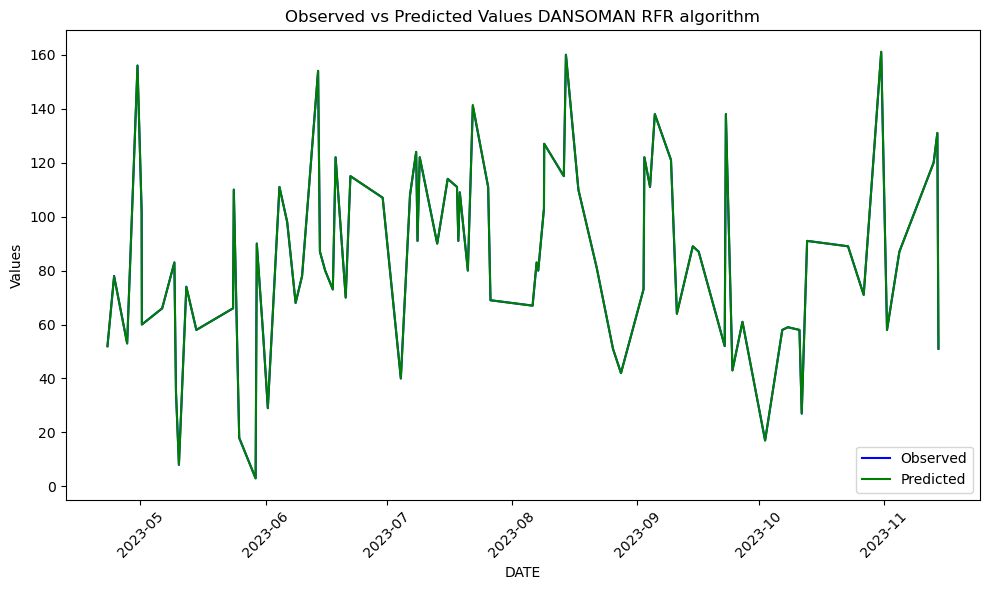
\includegraphics[width=\linewidth]{kawukudi rfr.png}
       
        \caption{ Predicted vs observed AQI RFR (Kawukudi) }
        \label{fig: RFR predicted vs observed AQI(Kawukudi)}
    \end{minipage}
\end{figure}
\subsection{CatBoost Regression}
The data is preprocessed and trained with the CatBoost Regression algorithm to predict the AQI. \\The table below shows the performance metrics after the model was configured on the Kawukudi dataset.
\begin{table}[H]
    \centering
    \begin{tabular}{|c|c|}
        \hline
        \textbf{Metric} & \textbf{Value} \\
        \hline
        MAE & 0.3326 \\
        \hline
        RMSE & 0.9665 \\
        \hline
        R-square & 0.9993\\
        \hline
    \end{tabular}
    \caption{Metrics for CatBoost Regression (Kawukudi)}
    \label{tab: CBR metrics(Kawukudi)}
\end{table}
\begin{figure}[H]
 \begin{minipage}{\linewidth}
        The figure below is a graph that shows how predicted values using the CatBoost Regression algorithm on the Kawukudi dataset were similar to observed values. Here the X-axis and Y-axis are Time and AQI values respectively.
        \vspace{0.5em} 
        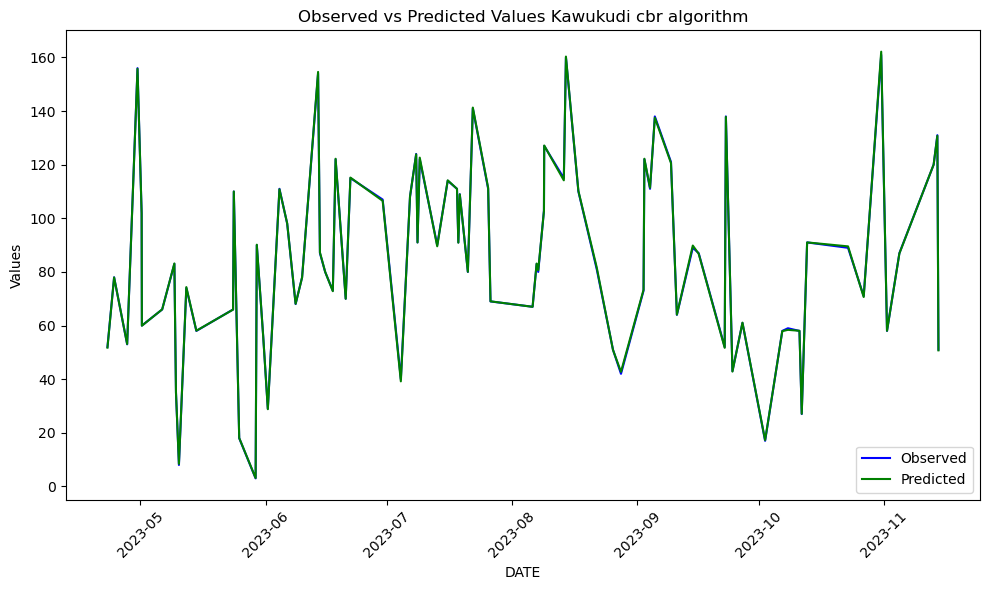
\includegraphics[width=\linewidth]{kawukudi cbr.png}
       
        \caption{ Predicted vs observed AQI CatBoost (Kawukudi) }
        \label{fig: CBR predicted vs observed AQI(Kawukudi)}
    \end{minipage}
\end{figure}
\vspace{-5mm}
\section{Korle Bu}
\label{korle bu}
\vspace{-5mm}
\subsection{Linear Regression}
\vspace{-5mm}
The data is preprocessed and trained with a linear regression algorithm to predict the AQI. The table below shows the performance metrics after the algorithm was tested.
\begin{table}[H]
    \centering
    \begin{tabular}{|c|c|}
        \hline
        \textbf{Metric} & \textbf{Value} \\
        \hline
        MAE & 4.5307 \\
        \hline
        RMSE & 8.8298 \\
        \hline
        R-square & 0.9341 \\
        \hline
    \end{tabular}
    \caption{Metrics for Linear Regression (Korle Bu)}
    \label{tab: Linear metrics(Korle Bu)}
\end{table}
\begin{figure}[H]
 \begin{minipage}{\linewidth}
        The figure below is a graph that shows how predicted values using the linear Regression algorithm on the Korle Bu dataset were similar to observed values. Here the X-axis and Y-axis are Time and AQI values respectively.
        \vspace{0.5em} 
        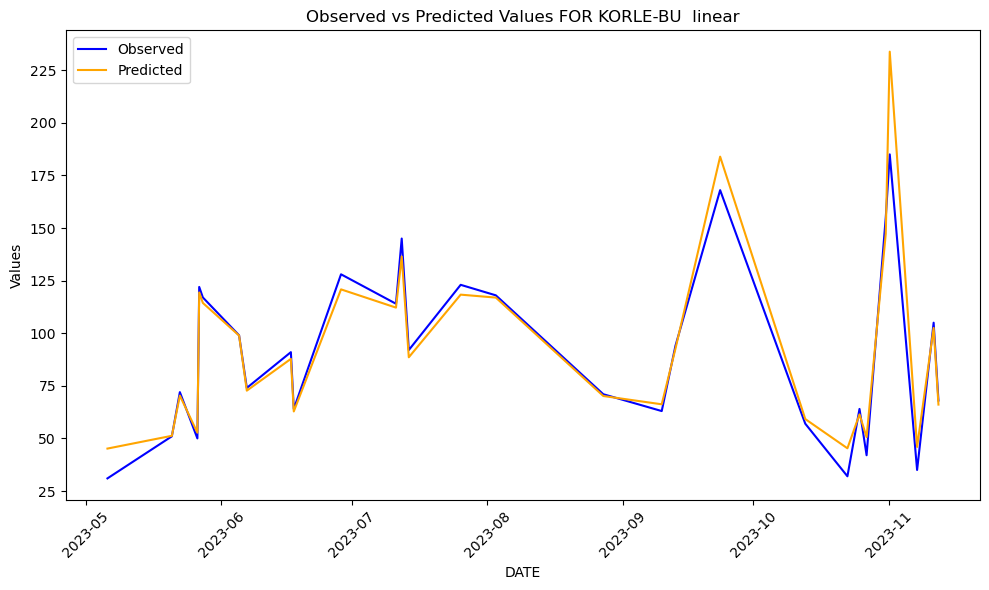
\includegraphics[width=\linewidth]{korle bu linear.png}
       
        \caption{ Predicted vs observed AQI Linear Regression (Korle Bu)}
        \label{fig: Linear predicted vs observed AQI(Korle Bu)}
    \end{minipage}
\end{figure}
\subsection{LASSO Regression}
The data is preprocessed and trained with the LASSO regression algorithm to predict the AQI. The table below shows the performance metrics after the LASSO regression model was configured on the Korle Bu dataset.
\begin{table}[H]
    \centering
    \begin{tabular}{|c|c|}
        \hline
        \textbf{Metric} & \textbf{Value} \\
        \hline
        MAE & 4.5922 \\
        \hline
        RMSE & 8.7301 \\
        \hline
        R-square & 0.9378 \\
        \hline
    \end{tabular}
    \caption{Metrics for LASSO Regression (Korle Bu)}
    \label{tab: LASSO metrics(Korle Bu)}
\end{table}
\begin{figure}[H]
 \begin{minipage}{\linewidth}
        The figure below is a graph that shows how predicted values using the LASSO Regression algorithm on the Korle Bu dataset were similar to observed values. Here the X-axis and Y-axis are Time and AQI values respectively.
        \vspace{0.5em} 
        \includegraphics[width=\linewidth]{korle bu LASSO.png}
       
        \caption{ Predicted vs observed AQI LASSO regression (Korle Bu)}
        \label{fig: LASSO predicted vs observed AQI(Korle Bu)}
    \end{minipage}
\end{figure}
\subsection{Ridge Regression}
The data was preprocessed and trained using the Ridge regression algorithm to predict the AQI. The table below presents the performance metrics after configuring the model on the Korle Bu dataset.
\begin{table}[H]
    \centering
    \begin{tabular}{|c|c|}
        \hline
        \textbf{Metric} & \textbf{Value} \\
        \hline
        MAE & 4.5908 \\
        \hline
        RMSE & 8.7301\\
        \hline
        R-square & 0.9378 \\
        \hline
    \end{tabular}
    \caption{Metrics for Ridge regression (Korle bu)}
    \label{tab: Ridge metrics(Korle Bu)}
\end{table}
\begin{figure}[H]
 \begin{minipage}{\linewidth}
        The figure below is a graph that shows how predicted values using the Ridge Regression algorithm on the Korle Bu dataset were similar to observed values. Here the X-axis and Y-axis are Time and AQI values respectively.
        \vspace{0.5em} 
        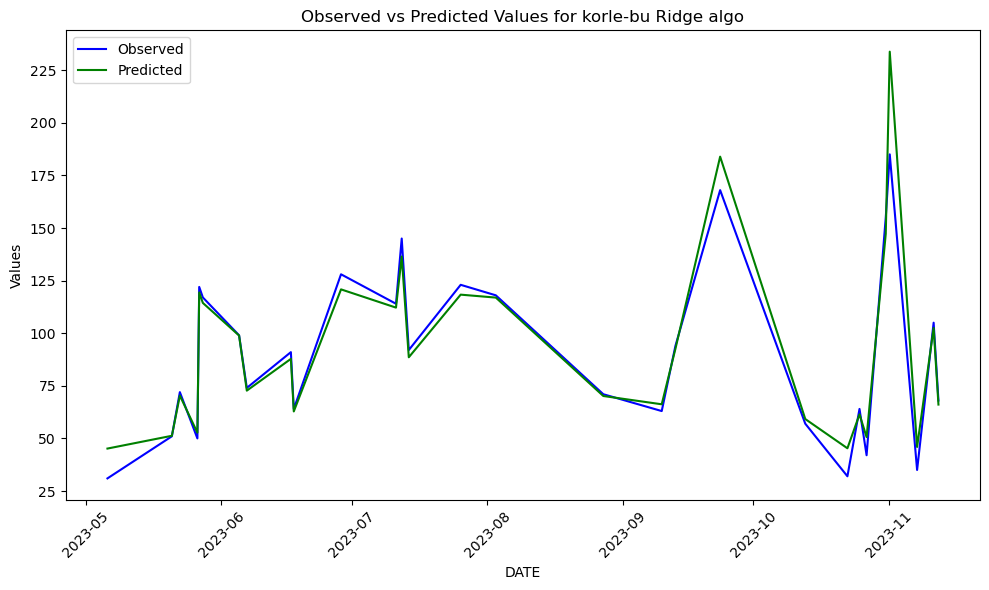
\includegraphics[width=\linewidth]{korle bu ridge.png}
       
        \caption{ Predicted vs observed AQI Ridge regression (Korle bu)}
        \label{fig: Ridge Predicted vs observed AQI(Korle Bu)}
    \end{minipage}
\end{figure}
\subsection{Support Vector Regression}
The data is preprocessed and trained with a Support Vector Regression algorithm to predict the AQI. The table below shows the performance metrics after the model was configured on the Korle Bu dataset.
\begin{table}[H]
    \centering
    \begin{tabular}{|c|c|}
        \hline
        \textbf{Metric} & \textbf{Value} \\
        \hline
        MAE & 0.5574 \\
        \hline
        RMSE & 2.0305 \\
        \hline
        R-square & 0.9965 \\
        \hline
    \end{tabular}
    \caption{Metrics for SVR (korle Bu)}
    \label{tab: SVR metrics(Korle Bu)}
\end{table}
\begin{figure}[H]
 \begin{minipage}{\linewidth}
        The figure below is a graph that shows how predicted values using the Support Vector Regression algorithm on the Korle Bu dataset were similar to observed values. Here the X-axis and Y-axis are Time and AQI values respectively.
        \vspace{0.5em} 
        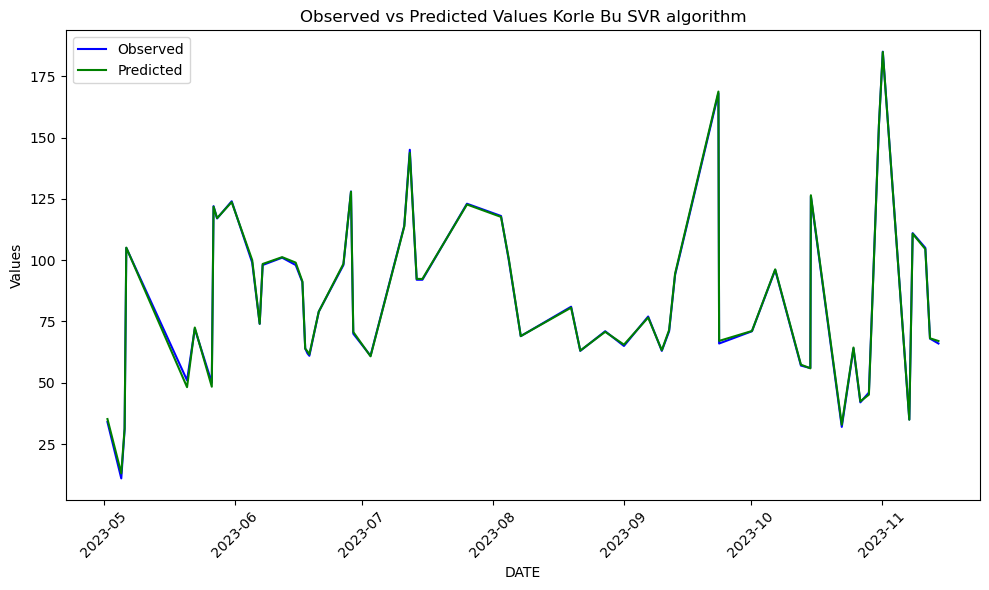
\includegraphics[width=\linewidth]{korle bu svr.png}
       
        \caption{ Predicted vs observed AQI SVR (korle Bu)}
        \label{fig: SVR Predicted vs observed AQI(Korle Bu)}
    \end{minipage}
\end{figure}
\subsection{Random Forest Regression}
The data is preprocessed and trained with the random forest regression algorithm to predict the AQI. The table below shows the performance metrics after the model was configured on the Korle Bu dataset.
\begin{table}[H]
    \centering
    \begin{tabular}{|c|c|}
        \hline
        \textbf{Metric} & \textbf{Value} \\
        \hline
        MAE & 0.0364 \\
        \hline
        RMSE & 0.2047\\
        \hline
        R-square & 1.0000\\
        \hline
    \end{tabular}
    \caption{Metrics for RFR (Korle Bu)}
    \label{tab: RFR metrics(Korle Bu)}
\end{table}
\begin{figure}[H]
 \begin{minipage}{\linewidth}
        The figure below is a graph that shows how predicted values using the Random Forest Regression algorithm on the Korle Bu dataset were very similar to observed values. Here the X-axis and Y-axis are Time and AQI values respectively.
        \vspace{0.5em} 
        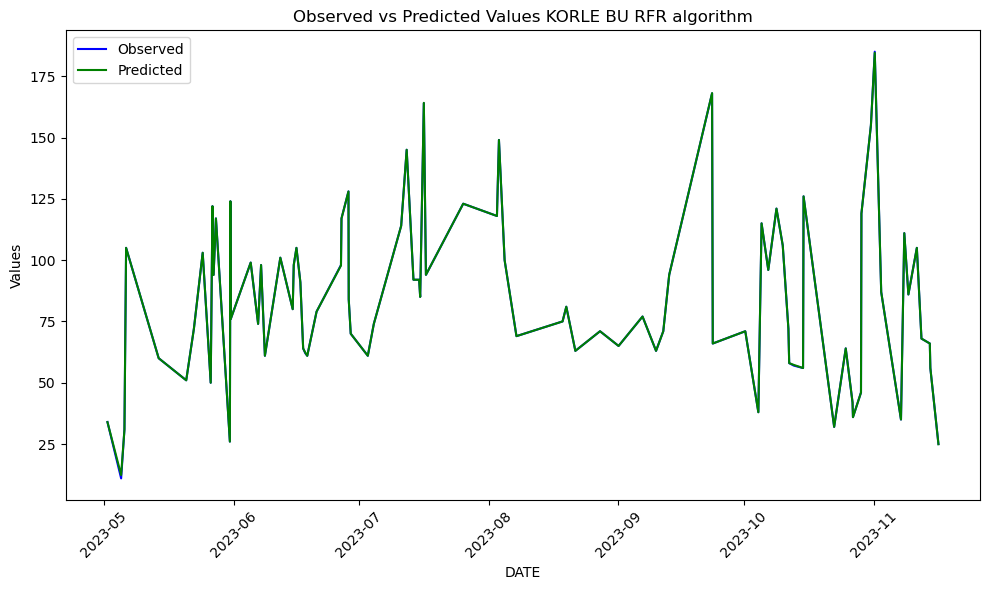
\includegraphics[width=\linewidth]{korle bu rfr.png}
       
        \caption{ Predicted vs observed AQI RFR (Korle Bu) }
        \label{fig: RFR Predicted vs observed AQI(Korle Bu)}
    \end{minipage}
\end{figure}
\subsection{CatBoost Regression}
The data is preprocessed and trained with the CatBoost Regression algorithm to predict the AQI. The table below shows the performance metrics after the model was configured on the Korle Bu dataset.
\begin{table}[H]
    \centering
    \begin{tabular}{|c|c|}
        \hline
        \textbf{Metric} & \textbf{Value} \\
        \hline
        MAE & 0.3249 \\
        \hline
        RMSE & 0.9310 \\
        \hline
        R-square & 0.9993\\
        \hline
    \end{tabular}
    \caption{Metrics for CatBoost regression (Korle Bu)}
    \label{tab: CBR metrics(korle Bu)}
\end{table}
\begin{figure}[H]
 \begin{minipage}{\linewidth}
        The figure below is a graph that shows how predicted values using the CatBoost Regression algorithm on the Korle Bu dataset were similar to observed values. Here the X-axis and Y-axis are Time and AQI values respectively.
        \vspace{0.5em} 
        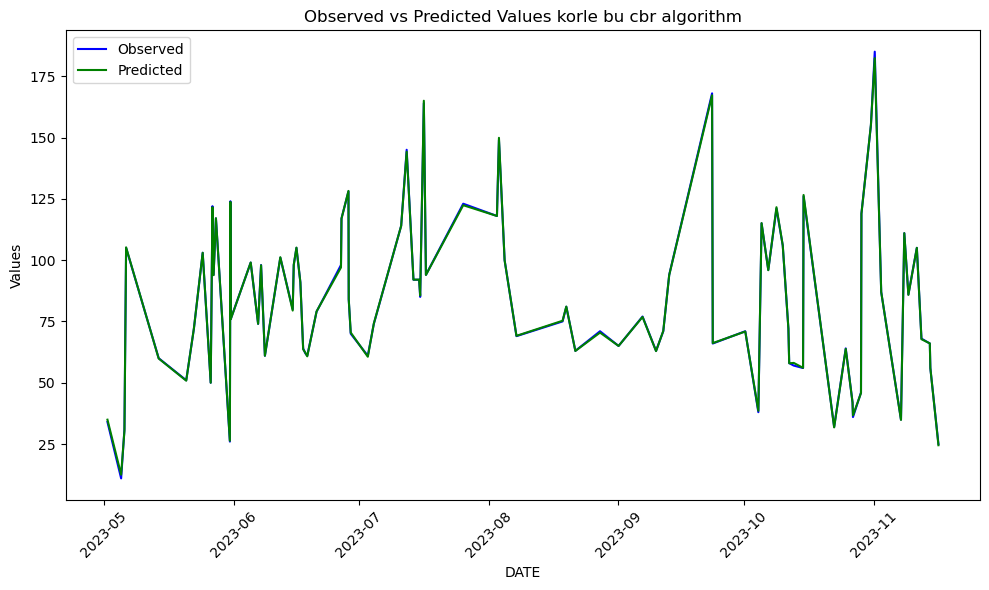
\includegraphics[width=\linewidth]{korle bu cbr.png}
       
        \caption{ Predicted vs observed AQI CatBoost regression (Korle Bu)}
        \label{fig: CBR Predicted vs observed AQI(Korle Bu)}
    \end{minipage}
\end{figure}

\vspace{-5mm} % Adjust the value to control the spacing
\section{Kwashieman}
\label{kwashieman}
\vspace{-5mm} % Adjust the value to control the spacing
\subsection{Linear Regression}
\vspace{-5mm} % Adjust the value to control the spacing
The data is preprocessed and trained with the linear regression algorithm to predict the AQI. The table below shows the performance metrics after the algorithm was tested.\\
\begin{table}[H]
    \centering
    \begin{tabular}{|c|c|}
        \hline
        \textbf{Metric} & \textbf{Value} \\
        \hline
        MAE & 6.7071 \\
        \hline
        RMSE & 9.7718 \\
        \hline
        R-square & 0.9276 \\
        \hline
    \end{tabular}
    \caption{Metrics for Linear regression (Kwashieman)}
    \label{tab: Linear metrics(Kwashieman)}
\end{table}
\begin{figure}[H]
 \begin{minipage}{\linewidth}
        The figure below is a graph that shows how predicted values using the linear Regression algorithm on the Kwashieman dataset were similar to observed values. Here the X-axis and Y-axis are Time and AQI values respectively.
        \vspace{0.5em} 
        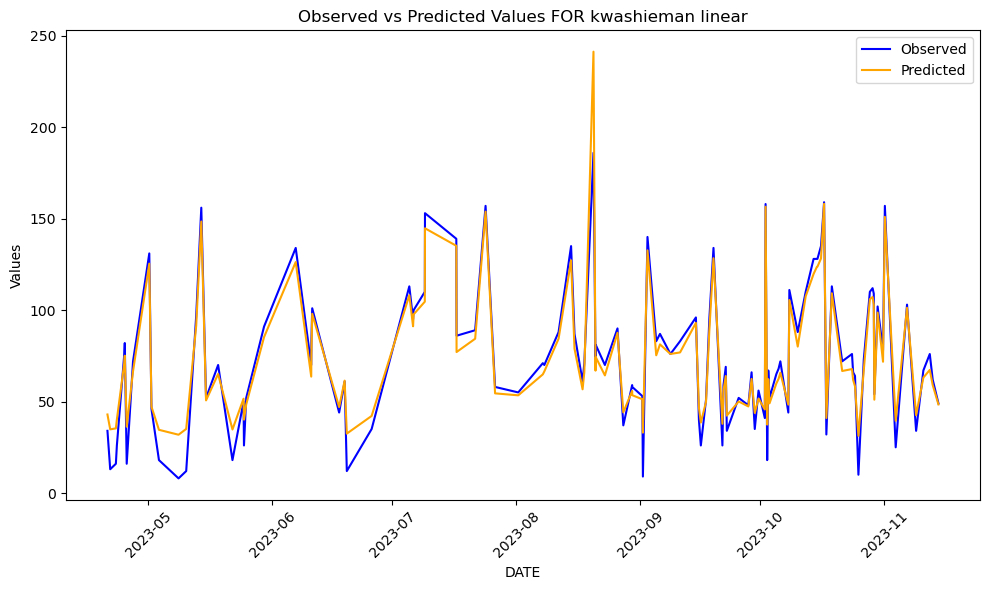
\includegraphics[width=\linewidth]{kwashieman linear.png}
       
        \caption{ Predicted vs observed AQI Linear regression (Kwashieman) }
        \label{fig: Linear predicted vs observed AQI(Kwashieman)}
    \end{minipage}
\end{figure}
%-----------------------------
\subsection{LASSO Regression}
The data is preprocessed and trained with the LASSO regression algorithm to predict the AQI. The table below shows the performance metrics after the LASSO regression model was configured on the Kwashieman dataset.
%%----------------------------------
\begin{table}[H]
    \centering
    \begin{tabular}{|c|c|}
        \hline
        \textbf{Metric} & \textbf{Value} \\
        \hline
        MAE & 6.8268 \\
        \hline
        RMSE & 10.6570 \\
        \hline
        R-square & 0.9158 \\
        \hline
    \end{tabular}
    \caption{Metrics for LASSO Regression (Kwashieman)}
    \label{tab:LASSO metrics(Kwashieman)}
\end{table}
\begin{figure}[H]
 \begin{minipage}{\linewidth}
        The figure below is a graph that shows how predicted values using the LASSO Regression algorithm on the Kwashieman dataset were similar to observed values. Here the X-axis and Y-axis are Time and AQI values respectively.
        \vspace{0.5em} 
        \includegraphics[width=\linewidth]{kwashieman LASSO.png}
       
        \caption{ Predicted vs observed AQI LASSO regression (Kwashieman)}
        \label{fig: LASSO predicted vs observed AQICkwashieman)}
    \end{minipage}
\end{figure}
\subsection{Ridge Regression}
The data was preprocessed and trained using the Ridge regression algorithm to predict the AQI. The table below presents the performance metrics after configuring the model on the kwashieman dataset.\\
\begin{table}[H]
    \centering
    \begin{tabular}{|c|c|}
        \hline
        \textbf{Metric} & \textbf{Value} \\
        \hline
        MAE & 6.8254 \\
        \hline
        RMSE & 10.6570\\
        \hline
        R-square & 0.9158 \\
        \hline
    \end{tabular}
    \caption{Metrics for Ridge regression (Kwashieman)}
    \label{tab: Ridge metrics(Kwashieman)}
\end{table}
\begin{figure}[H]
 \begin{minipage}{\linewidth}
        The figure below is a graph that shows how predicted values using the Ridge Regression algorithm on the Kwashieman dataset were similar to observed values. Here the X-axis and Y-axis are Time and AQI values respectively.
        \vspace{0.5em} 
        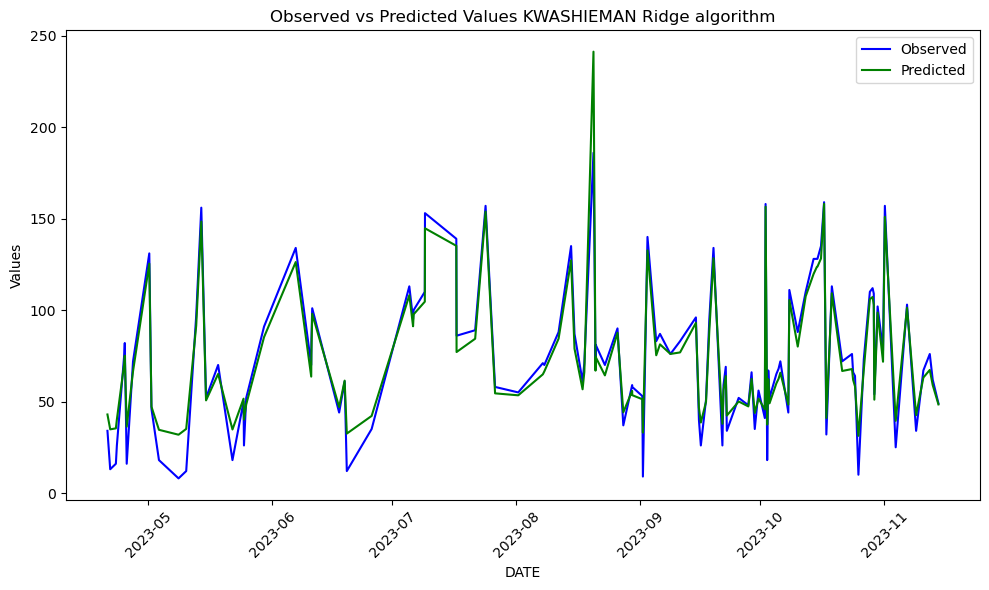
\includegraphics[width=\linewidth]{kwashieman ridge.png}
       
        \caption{ Predicted vs observed AQI Ridge regression (Kwashieman)}
        \label{fig: Ridge predicted vs observed AQI(Kwashieman)}
    \end{minipage}
\end{figure}
%%------------
\subsection{Support Vector Regression}
The data is preprocessed and trained with a Support Vector Regression algorithm to predict the AQI. The table below shows the performance metrics after configuring the Kwashieman dataset's model.
\begin{table}[H]
    \centering
    \begin{tabular}{|c|c|}
        \hline
        \textbf{Metric} & \textbf{Value} \\
        \hline
        MAE & 0.8060 \\
        \hline
        RMSE & 5.2848 \\
        \hline
        R-square & 0.9788 \\
        \hline
    \end{tabular}
    \caption{Metrics for SVR (Kwashieman)}
    \label{tab: SVR metrics (Kwashieman)}
\end{table}
\begin{figure}[H]
 \begin{minipage}{\linewidth}
        The figure below is a graph that shows how predicted values using the Support Vector Regression algorithm on the Kwashieman dataset were similar to observed values. Here the X-axis and Y-axis are Time and AQI values respectively.
        \vspace{0.5em} 
        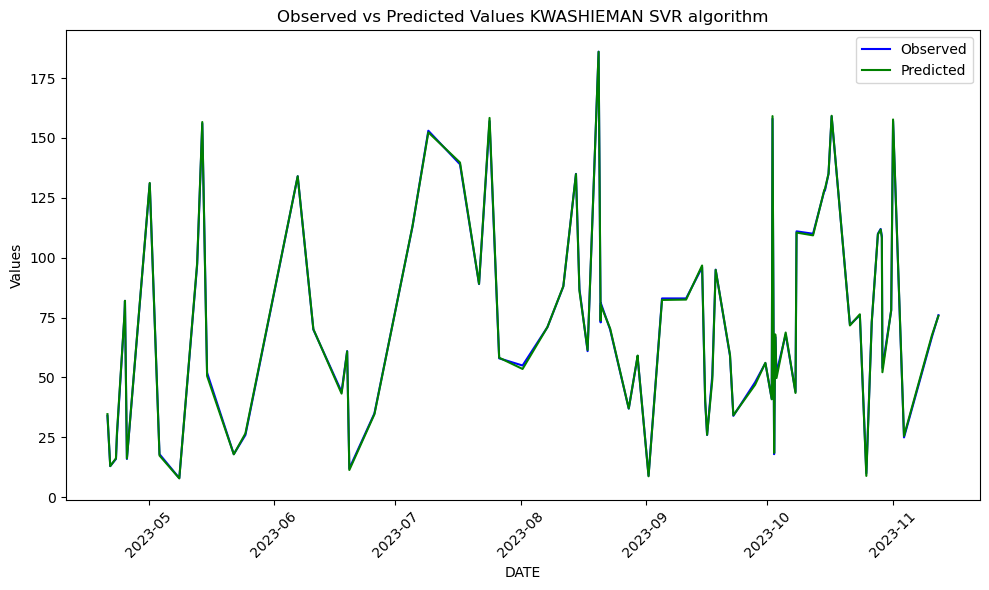
\includegraphics[width=\linewidth]{kwashieman svr.png}
       
        \caption{ Predicted vs observed AQI SVR (Kwashieman)}
        \label{fig: SVR Predicted vs observed AQI (Kwashieman)}
    \end{minipage}
\end{figure}
%--
\subsection{Random Forest Regression}
The data is preprocessed and trained with the random forest regression algorithm to predict the AQI. The table below shows the performance metrics after configuring the Kwashieman dataset's model.
\begin{table}[H]
    \centering
    \begin{tabular}{|c|c|}
        \hline
        \textbf{Metric} & \textbf{Value} \\
        \hline
        MAE & 0.0233 \\
        \hline
        RMSE & 0.1274\\
        \hline
        R-square & 1.0000\\
        \hline
    \end{tabular}
    \caption{Metrics for Random Forest Regression (Kwashieman)}
    \label{tab: RFR metrics (Kwashieman)}
\end{table}
\begin{figure}[H]
 \begin{minipage}{\linewidth}
        The figure below is a graph that shows how predicted values using the Random Forest Regression algorithm on the Kwashieman dataset were very similar to observed values. Here the X-axis and Y-axis are Time and AQI values respectively.
        \vspace{0.5em} 
        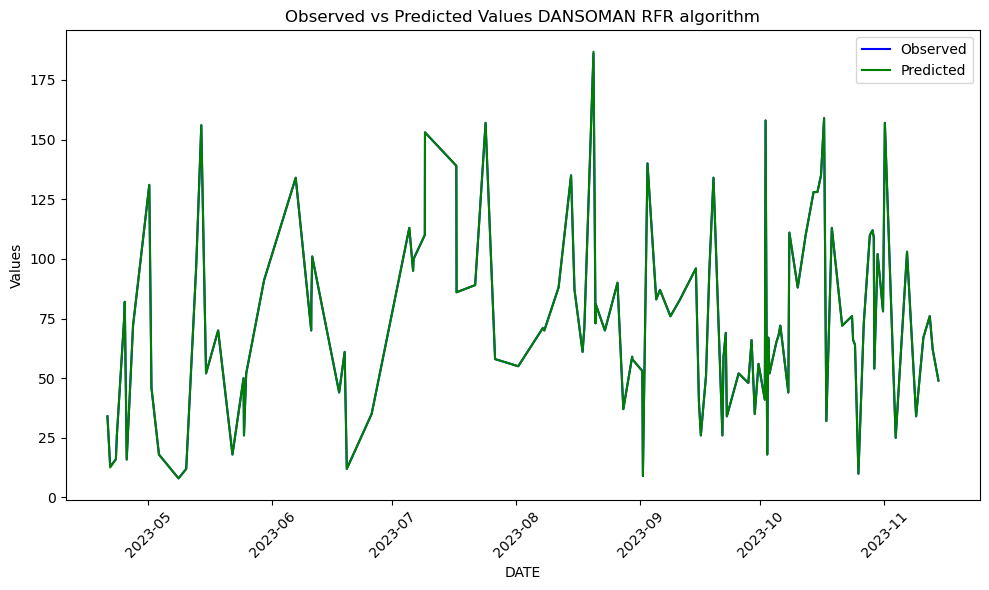
\includegraphics[width=\linewidth]{kwashieman rfr.png}
       
        \caption{ Predicted vs observed AQI RFR (Kwashieman)}
        \label{fig: RFR Predicted vs observed AQI (Kwashieman)}
    \end{minipage}
\end{figure}
%%--------------
\subsection{CatBoost  Regression}
The data is preprocessed and trained with the CatBoost Regression algorithm to predict the AQI. The table below shows the performance metrics after configuring the Kwashieman dataset's model.
\begin{table}[H]
    \centering
    \begin{tabular}{|c|c|}
        \hline
        \textbf{Metric} & \textbf{Value} \\
        \hline
        MAE & 0.2836 \\
        \hline
        RMSE & 0.8099\\
        \hline
        R-square & 0.9995\\
        \hline
    \end{tabular}
    \caption{ Metrics for CatBoost regression (Kwashieman)}
    \label{tab: CBR metrics (Kwashieman)}
\end{table}
\begin{figure}[H]
 \begin{minipage}{\linewidth}
        The figure below is a graph that shows how predicted values using the CatBoost Regression algorithm on the Kwashieman dataset were similar to observed values. Here the X-axis and Y-axis are Time and AQI values respectively.
        \vspace{0.5em} 
        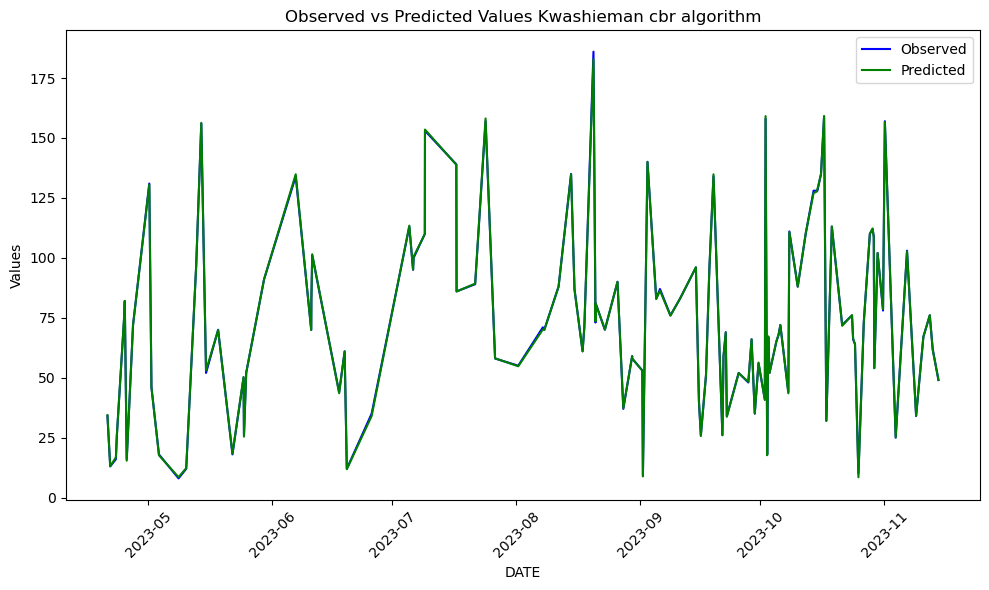
\includegraphics[width=\linewidth]{kwashieman cbr.png}
       
        \caption{ Predicted vs observed AQI CatBoost regression (Kwashieman)}
        \label{fig: CBR predicted v observed (Kwashieman)}
    \end{minipage}
\end{figure}
%---------------------------------------------
\section{Accra}
\label{chp:numericalresults}
 %---------------------------------------------
In this section, we showcase the numerical results derived from utilizing Linear regression, LASSO regression, Ridge regression, Support vector regression, Random Forest regression, and Catboost regression algorithms to forecast the Air Quality Index (AQI) with all five datasets from some neighborhoods in Accra. Careful preprocessing was conducted to maintain the data's quality and pertinence. Our main objective is to assess the trained model's performance and comprehend its predictive effectiveness. The subsequent figures display the performance metrics, offering insights into the model's accuracy.
\begin{table}[H]
    \centering
    \begin{tabular}{|c|c|c|c|}
        \hline
        Model & MAE & RMSE & $R^2$ score \\
        \hline
        Linear Regression & 6.7071 & 9.7718 & 0.9276 \\
        \hline
        LASSO Regression & 6.8268 & 10.6570 & 0.9158 \\
        \hline
        Ridge Regression & 6.8254 & 10.6570 & 0.9158 \\
        \hline
        Support Vector Regression & 0.8060 & 5.2848 & 0.9788 \\
        \hline
        Random Forest Regression & 0.0233 & 0.1274 & 1.0000 \\
        \hline
        CatBoost Regression &  0.2836 & 0.8099 &  0.9995 \\\hline
    \end{tabular}
    \caption{Kwashieman}
   \label{tab: all algorithms on Kwashieman}
\end{table}
\begin{table}[H]
    \centering
    \begin{tabular}{|c|c|c|c|}
        \hline
        Model & MAE & RMSE & $R^2$ score \\
        \hline
        Linear Regression & 4.5307 & 8.8298 & 0.9341 \\
        \hline
        LASSO Regression & 4.5922 & 8.7301 & 0.9379 \\
        \hline
        Ridge Regression & 4.5908 & 8.7301 & 0.9378 \\
        \hline
        Support Vector Regression & 0.5574 & 2.0305 & 0.9965 \\
        \hline
        Random Forest Regression & 0.0364 & 0.2047 & 1.0000 \\
        \hline
        CatBoost Regression & 0.3249 & 0.9310 & 0.9993 \\\hline
    \end{tabular}
    \caption{Korle Bu}
   \label{tab: all algorithms on Korle Bu}
\end{table}
\begin{table}[H]
    \centering
    \begin{tabular}{|c|c|c|c|}
        \hline
        Model & MAE & RMSE & $R^2$ score \\
        \hline
        Linear Regression & 4.8870 & 8.1989 & 0.9435 \\
        \hline
        LASSO Regression & 4.9546 & 8.1768 & 0.9457 \\
        \hline
        Ridge Regression & 4.9538 & 8.1768 & 0.9457 \\
        \hline
        Support Vector Regression & 0.7681 & 4.7741 & 0.809 \\
        \hline
        Random Forest Regression & 0.03361 & 0.2948 & 0.9999 \\
        \hline
        CatBoost Regression & 0.3058 & 1.0185 & 0.9991 \\\hline
    \end{tabular}
    \caption{Kanda}
   \label{tab: all algorithms on Kanda}
\end{table}
\begin{table}[H]
    \centering
    \begin{tabular}{|c|c|c|c|}
        \hline
        Model & MAE & RMSE & $R^2$ score \\
        \hline
        Linear Regression &7.8628 & 12.8249 & 0.8839 \\
        \hline
        LASSO Regression & 7.8263 & 12.7065 & 0.8861 \\
        \hline
        Ridge Regression & 7.8249 & 12.7065 & 0.8861 \\
        \hline
        Support Vector Regression & 1.0098 & 6.7301 & 0.9680 \\
        \hline
        Random Forest Regression & 0.0415 & 0.2702 & 0.9999 \\
        \hline
        CatBoost Regression & 0.3326 & 0.9665 & 0.9993 \\\hline
    \end{tabular}
    \caption{Kawukudi}
   \label{tab: all algorithms combined on Kawukudi}
\end{table}
\begin{table}[H]
    \centering
    \begin{tabular}{|c|c|c|c|}
        \hline
        Model & MAE & RMSE & $R^2$ score \\
        \hline
        Linear Regression & 6.3633 & 8.6067 & 0.9455 \\
        \hline
        LASSO Regression & 6.4828 & 9.6909 & 0.9311 \\
        \hline
        Ridge Regression & 6.4812 & 9.6909 & 0.9311 \\
        \hline
        Support Vector Regression & 0.7714 & 2.9456 & 0.9936 \\
        \hline
        Random Forest Regression & 0.0262 & 0.1185 & 1.0000 \\
        \hline
        CatBoost Regression & 0.2947 & 0.7402 & 0.9992 \\\hline
    \end{tabular}
    \caption{Dansoman}
   \label{tab: all algorithms' metrics on Dansoman}
\end{table}
\begin{table}[H]
    \centering
    \begin{tabular}{|c|c|c|c|}
        \hline
        Model & MAE & RMSE & $R^2$ score \\
        \hline
        Linear Regression & 6.3633 & 8.6067 & 0.9455 \\
        \hline
        LASSO Regression & 6.4666 & 10.6246 & 0.9179 \\
        \hline
        Ridge Regression & 6.4652 & 10.6246 &  0.9179 \\
        \hline
        Support Vector Regression &  0.5726 & 2.5162 & 0.9954 \\
        \hline
        Random Forest Regression & 0.0061 & 0.0736 & 1.0000 \\
        \hline
        CatBoost Regression & 0.2787 & 1.0418 & 1.0000 \\\hline
    \end{tabular}
    \caption{Accra}
   \label{tab: all areas}
\end{table}
%--------------------------------------------------------------
%\newpage
\begin{figure}[H]
 \begin{minipage}{\linewidth}
        The graph below illustrates the mean absolute error (MAE) for all algorithms when trained on datasets from various areas in Accra.
        \vspace{0.5em} 
        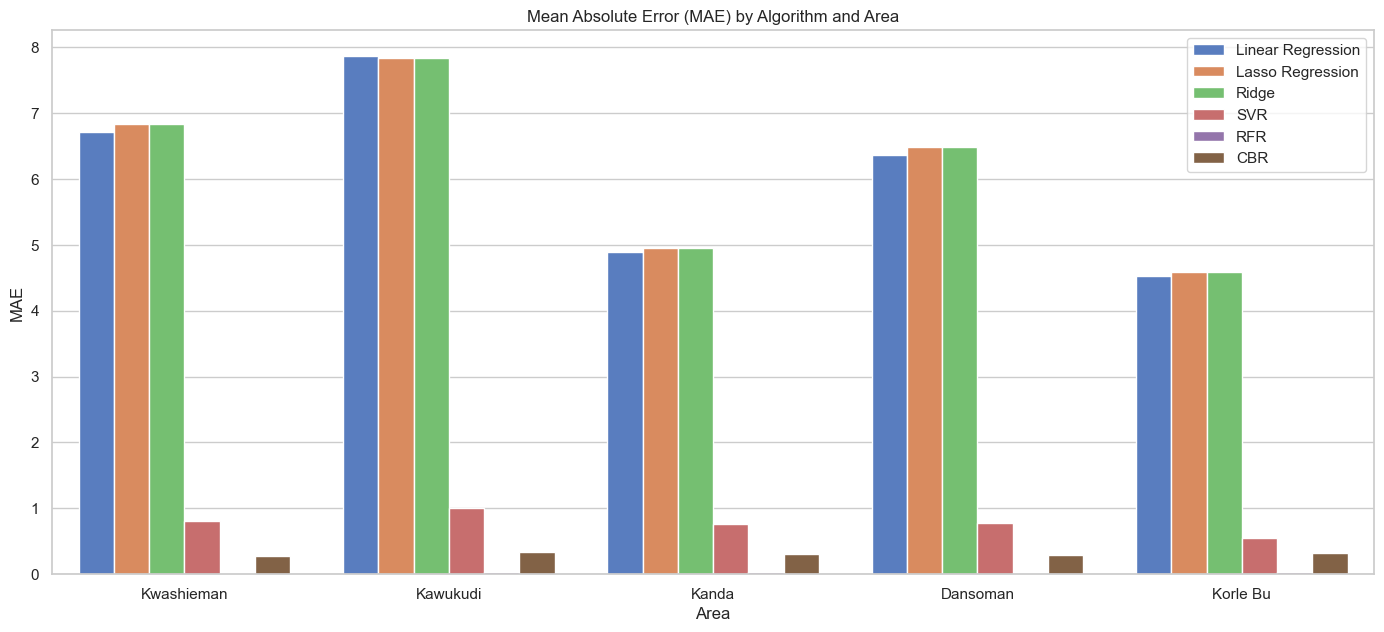
\includegraphics[width=\linewidth]{MAE of all areas.png}
       
        \caption{ Multiple bar chart of MAE for all algorithms}
        \label{fig: Bar chart of the MAE for all algorithms}
    \end{minipage}
\end{figure}
\begin{figure}[H]
 \begin{minipage}{\linewidth}
        The graph below illustrates the root mean squared error (RMSE) for all algorithms when trained on datasets from various areas in Accra.
        \vspace{0.5em} 
        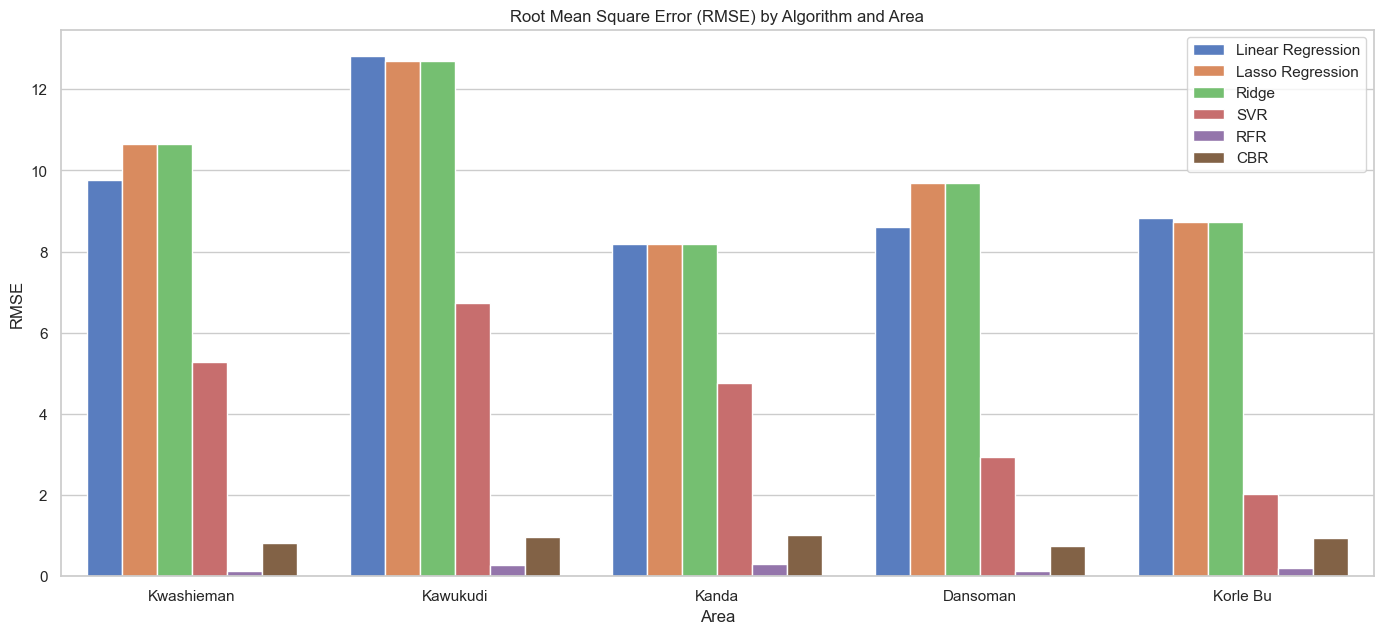
\includegraphics[width=\linewidth]{RMSE of all areas.png}
       
        \caption{ Multiple bar chart of the RMSE for all algorithms}
        \label{fig: Bar chart of the RMSE for all algorithms}
    \end{minipage}
\end{figure}
\begin{figure}[H]
 \begin{minipage}{\linewidth}
        The graph below illustrates the R-squared score ($R^{2}$) for all algorithms when trained on datasets from various areas in Accra.
        \vspace{0.5em} 
        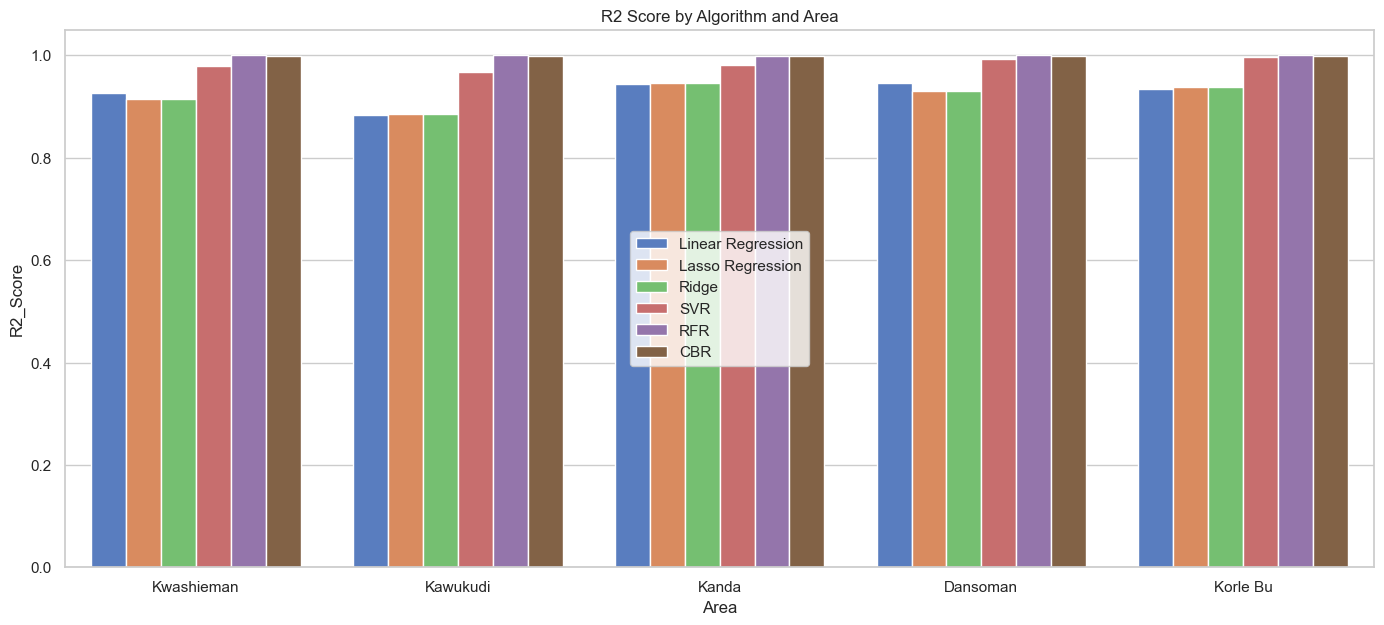
\includegraphics[width=\linewidth]{r2 score.png}
       
        \caption{ Multiple Bar chart of the $R^{2}$ score for all algorithms}
        \label{fig: Bar chart of the $R^{2}$ score  for all algoritms}
    \end{minipage}
\end{figure}
\section{Discussion}
\label{discussion}
The study aimed to predict the Air Quality Index (AQI) using various machine learning algorithms, including Linear Regression, LASSO Regression, Ridge Regression, Support Vector Regression (SVR), CatBoost Regression, and Random Forest Regression. Our analysis focused on evaluating the performance of these models using metrics such as $R^{2}$ score, Mean Absolute Error (MAE), and Root Mean Square Error (RMSE). This section discusses the implications of our findings, compares them with existing literature, and addresses the strengths and limitations of our approach.\\
 In the above multiple bar graphs, the X-axis represents all the algorithms and areas in Accra and the Y-axis represents the performance metrics. By observing the charts, when compared to all algorithms the model has the lowest MAE, lowest RMSE, and highest $R^{2}$ score when built using Random Forest Regression. This means that Random Forest Regression is good for forecasting the AQI.
%--------------------------------------------------------------
 \chapter{Conclusion and Recommendation}
 \label{ch5}
%\vspace{\baselineskip}
%%%%%%%%%--------------
\section{Conclusion}
\label{conclusion}
In this study, six supervised machine learning algorithms were trained and tested using datasets from five different areas in Accra. All datasets underwent rigorous preprocessing before being trained using each algorithm. Performance was evaluated using three metrics: Mean Absolute Error (MAE), Root Mean Square Error (RMSE), and the $R^2$ score. 
Our findings indicate that Random Forest Regression consistently outperformed the other models, achieving the lowest MAE and RMSE, as well as the highest $R^2$ score across all regions considered in this research. This superior performance can be attributed to the algorithm's ability to handle non-linear relationships and interactions between features effectively, providing robust and accurate predictions.
%%%%%%%%%--------------
\section{Recommendation}
\label{recommendation}
Incorporation of Additional Features for Enhanced Predictive Power. To enrich the predictive accuracy of AQI  models, it is recommended to integrate supplementary features beyond pollutant concentrations alone. Specifically, the inclusion of meteorological data such as temperature, humidity, and wind speed can provide crucial insights into atmospheric dynamics affecting pollutant dispersion and concentration levels. These variables, known to influence air quality patterns, enable a more comprehensive understanding of AQI fluctuations across different temporal and spatial scales.

Furthermore, considering geographical factors such as altitude and proximity to industrial zones can significantly augment model robustness. Altitude affects atmospheric pressure and temperature gradients, which in turn impact pollutant dispersion and transformation processes. Meanwhile, proximity to industrial areas introduces localized emissions that can variably influence AQI readings.
By incorporating these additional features into AQI prediction models, the models can capture complex interactions between atmospheric conditions and pollutant sources and enhance their predictive capability across diverse environmental contexts. This approach improves the accuracy of forecasting future AQI levels and supports more informed decision-making for environmental management and public health interventions.
%-----------------------------------------
\begin{thebibliography}{99}
\bibitem{Landrigan2018}
    Landrigan, P. J., et al. (2018). The Lancet Commission on pollution and health. The Lancet, 391(10119), 462-512.
\bibitem{Guo2017}
    Guo, H., Wang, Y., Zhang, H., Wang, L., Liu, H., & Zhang, X. (2017). Source apportionment of fine particulate matter in Beijing, China: Insights into the
contributions of biomass burning, motor vehicles, and coal combustion. At￾mospheric Chemistry and Physics, 17(11), 7485-7498.
\bibitem{Burnett2018}
    Burnett, R. T., et al. (2018). Global estimates of mortality associated with long-term exposure to outdoor fine particulate matter. Proceedings of the Na￾tional Academy of Sciences, 115(38), 9592-9597.
\bibitem{Ramanathan2008}
    Ramanathan, V., & Feng, Y. (2008). Air pollution, greenhouse gases and climate change: Global and regional perspectives. Atmospheric Environment,
43(1), 37-50
\bibitem{Huang2015}
    Huang, J., Zhang, X., Zhang, Q., & Yang, Y. (2015). A review of air quality index and air quality health assessment. Environmental International, 74, 97-108.
\bibitem{Miller2020}
Miller, R. L., & Liao, K. (2020). Public awareness and engagement in air quality management: The role of community-based programs. Environmental
Science & Policy, 108, 1-11.
\bibitem{Strickland2020}
    Strickland, J. R., & Darrow, E. E. (Year). The Air Quality Index (AQI) and its role in public health: A review. Journal of Environmental Health.
\bibitem{shishegaran2020}
    A. Shishegaran, M. Saeedi, A. Kumar, and H. Ghiasinejad, "Prediction of air quality in Tehran by developing the non-linear ensemble model," \textit{Journal of Cleaner Production}, vol. 259, p. 120825, 2020.
\bibitem{londhe2021}
    M. Londhe, "Data mining and machine learning approach for air quality index prediction," \textit{International Journal of Engineering and Applied Physics}, vol. 1, no. 2, pp. 136-153, 2021.
\bibitem{janarthanan2021}
    R. Janarthanan, P. Partheeban, K. Somasundaram, and P. N. Elamparithi, "A deep learning approach for prediction of air quality index in a metropolitan city," \textit{Sustainable Cities and Society}, vol. 67, p. 102720, 2021.
\bibitem{gore2017}
    R. W. Gore and D. S. Deshpande, "An approach for classification of health risks based on air quality levels," in \textit{Proceedings of the 2017 1st International Conference on Intelligent Systems and Information Management (ICISIM)}, Aurangabad, India, 2017, pp. 58-61.
\bibitem{zhao2020}
    X. Zhao, M. Song, A. Liu, Y. Wang, T. Wang, and J. Cao, "Data-Driven temporal-spatial model for the prediction of AQI in Nanjing," \textit{Journal of Artificial Intelligence and Soft Computing Research}, vol. 10, no. 4, pp. 255-270, 2020.
\bibitem{kumar2011}
    Anikender Kumar and Pramila Goyal, "Forecasting of Air Quality Index in Delhi using Principal Component Regression and Multiple Linear Regression Models," 2011.
\bibitem{castelli2020} 
    Mauro Castelli, F. M. Clemente, A. Popovič, S. Silva, and L. Vanneschi, "A machine learning approach to predict air quality in California," Complexity, vol. 2020, 2020.
\bibitem{liu2017} 
    Bing-chun Liu et al., "Multi-dimensional collaborative SVR model for air quality prediction," 2017.
\bibitem{sethi2021} 
    Jasleen Kaur Sethi and Mamta Mittal, "Correlation based Adaptive LASSO regression method for air quality index prediction," 2021.
\bibitem{li2021} 
    Chenchen Li et al., "Comparison of supervised machine learning algorithms for predicting air quality index," 2021.
\bibitem{linear_regression}
    James, G., Witten, D., Hastie, T., \& Tibshirani, R. (2013). \textit{An Introduction to Statistical Learning}. Springer. Chapter 3: Linear Regression.
\bibitem{LASSO_regression}
    Tibshirani, R. (1996). Regression Shrinkage and Selection via the LASSO. 
    \textit{Journal of the Royal Statistical Society: Series B (Methodological)}, 58(1), 267-288.
\bibitem{ridge_regression}
    Hoerl, A. E., \& Kennard, R. W. (1970). Ridge Regression: Biased Estimation for Nonorthogonal Problems. \textit{Technometrics}, 12(1), 55-67.
\bibitem{svr}
    Drucker, H., Burges, C. J. C., Kaufman, L., Smola, A., \& Vapnik, V. (1997). Support Vector Regression Machines. \textit{Advances in Neural Information Processing Systems}, 9, 155-161.
\bibitem{catboost}
    Prokhorenkova, L., Gusev, G., Vorobev, A., Dorogush, A. V., \& Gulin, A. (2018). CatBoost: Unbiased Boosting with Categorical Features. \textit{Advances in Neural Information Processing Systems}, 31, 6638-6648.  
\bibitem{random_forest}
    Breiman, L. (2001). Random Forests. \textit{Machine Learning}, 45(1), 5-32.
\bibitem{leong2019prediction}
    Leong, W. C., Kelani, R. O., \& Ahmad, Z. (2019). Prediction of air pollution index (API) using support vector machine (SVM). Journal of Environmental Chemical Engineering, 7(4), 103141.
\bibitem{hajek2015predicting}
    Hajek, P., \& Olej, V. (2015). Predicting common air quality index-the case of Czech microregions. Aerosol and Air Quality Research, 15(2), 544-555.
\bibitem{breiman2001random}
    Breiman, L. (2001). Random forests. Machine Learning, 45(1), 5-32.
\bibitem{liaw2002classification}
    Liaw, A., \& Wiener, M. (2002). Classification and regression by randomForest. R News, 2(3), 18-22.
\bibitem{zhang2017hybrid}
    Zhang, X., Tang, L., Luo, L., \& Liang, J. (2017). A hybrid air quality early-warning system based on machine learning and multiple linear regression. Atmospheric Environment, 166, 98-105.
\bibitem{jiang2020hybrid}
    Jiang, Y., Bai, Y., Yang, C., \& Tang, T. (2020). A hybrid model for short-term air quality prediction. Atmospheric Pollution Research, 11(1), 218-229.
\bibitem{pai1997simulation}
    Pai, P., Karamchandani, P., \& Seifneur, C. (1997). Simulation of the regional atmospheric transport and fate of mercury using a comprehensive eulerian model. Atmospheric Environment, 31, 2717–2732.
\bibitem{gaikar2023prediction}
    Gaikar, D., Patel, U., Vispute, O., Singh, S., \& Sanghvi, T. (2023). Prediction of Air Quality Index using Random Forest Algorithm. \textit{International Research Journal of Engineering and Technology}, 10(4), 1248-1252.
\bibitem{lalitkishore2023application}
    Lalitkishore, N., \& Manoharan, S. (2023). Application of Catboost algorithm as a predictive tool in a CNC turning process. \textit{International Journal of Advance Research, Ideas and Innovations in Technology}, 9(5), 145-151.
\bibitem{prokhorenkova2018catboost}
    Prokhorenkova, L., Gusev, G., Vorobev, A., Dorogush, A. V., \& Gulin, A. (2018). CatBoost: unbiased boosting with categorical features. \textit{Advances in neural information processing systems}, 31.
\bibitem{chakraborty2021application}
    Chakraborty, S., \& Bhattacharya, S. (2021). Application of XGBoost algorithm as a predictive tool in a CNC turning process. \textit{Reports in Mechanical Engineering}, 2(1), 190-201.
\bibitem{lee1996adaptive}
    Lee, B. Y., \& Tarng, Y. S. (1996). Adaptive modeling and optimization of machining processes.  \textit{International Journal of Production Research}, 34(7), 1883-1898.
\bibitem{hochreiter1997long}
    Hochreiter, S., \& Schmidhuber, J. (1997). Long short-term memory. \textit{Neural computation}, 9(8), 1735-1780.
\bibitem{snoek2012practical}
    Snoek, J., Larochelle, H., \& Adams, R. P. (2012). Practical bayesian optimization of machine learning algorithms. \textit{Advances in neural information processing systems}, 25.
\bibitem[Gupta et al., 2023]{gupta2023}
    Gupta, S., Kumar, A., \& Sharma, P. (2023). Prediction of Air Quality Index Using Machine Learning Techniques: A Comparative Analysis. \textit{Journal of Environmental and Public Health}, \textit{2023}, 1-12. 
    Kumar, V., \& Minz, S. (2014). Feature selection: A literature review. \textit{SmartCR}, 4(3), 211-229.
\bibitem{Wang2016}
    Wang, S., Peng, J., \& Li, J. (2016). Integration of filter and wrapper methods for feature selection in high-dimensional datasets. \textit{IEEE Transactions on Systems, Man, and Cybernetics: Systems}, 46(3), 315-326.
\bibitem{Tibshirani1996}
    Tibshirani, R. (1996). Regression shrinkage and selection via the LASSO. \textit{Journal of the Royal Statistical Society: Series B (Methodological)}, 58(1), 267-288.
\bibitem{Melkumova2017}
    Melkumova, L., \& Shatskikh, S. (2017). Comparing Ridge and LASSO estimators for data analysis. \textit{Procedia Engineering}, 201, 746-755.
\bibitem{Qian2013}
    Qian, J., \& Yang, L. (2013). Adaptive LASSO for sparse high-dimensional regression models. \textit{Statistics and Its Interface}, 6(3), 357-370.
\bibitem{Sethi2021}
    Sethi, J. K., \& Mittal, M. (2021). An efficient correlation based adaptive LASSO regression method for air quality index prediction. \textit{Earth Science Informatics}. https://doi.org/10.1007/s12145-021-00618-1
\bibitem{breiman1996a}
    Breiman, L. (1996a). Bagging predictors. \textit{Machine Learning, 26}(2), 123-140.
\bibitem{breiman1996b}
    Breiman, L. (1996b). Out-of-bag estimation, ftp.stat.berkeley.edu/pub/users/breiman/OOBestimation.ps
\bibitem{breiman1999}
    Breiman, L. (1999). Using adaptive bagging to debias regressions. \textit{Technical Report 547, Statistics Dept. UCB}.
\bibitem{breiman2000}
    Breiman, L. (2000). Some infinity theory for predictor ensembles. \textit{Technical Report 579, Statistics Dept. UCB}.
\bibitem{schapire1998}
    Schapire, R., Freund, Y., Bartlett, P., \& Lee, W. (1998). Boosting the margin: A new explanation for the effectiveness of voting methods. \textit{Annals of Statistics, 26}(5), 1651-1686.
\bibitem{liu2019air}
    Liu, H., Li, Q., Yu, D., \& Gu, Y. (2019). Air quality index and air pollutant concentration prediction based on machine learning algorithms. Applied Sciences, 9(19), 4069.
\bibitem{perez2000prediction}
    P'erez, P., Trier, A., \& Reyes, J. (2000). Prediction of PM$_{2.5}$ concentrations several hours in advance using neural networks in Santiago, Chile. Atmospheric Environment, 34(8), 1189-1196.
\bibitem{corani2005air}
    Corani, G. (2005). Air quality prediction in Milan: Feed-forward neural networks, pruned neural networks and lazy learning. Ecological Modelling, 185(2-4), 513-529.
\bibitem{biancofiore2017recursive}
    Biancofiore, F., Busilacchio, M., Verdecchia, M., Tomassetti, B., Aruffo, E., Bianco, S.,\& Di Carlo, P. (2017). Recursive neural network model for analysis and forecast of PM$_{10}$ and PM${2.5}$. Atmospheric Pollution Research, 8(4), 652-659.
\bibitem{zhu2017daily}
    Zhu, S., Lian, X., Liu, H., Hu, J., Wang, Y., \& Che, J. (2017). Daily air quality index forecasting with hybrid models: A case in China. Environmental Pollution, 231, 1232-1244.
\bibitem[Friedman et al.(2010)Friedman, Hastie, and Tibshirani]{friedman2010regularization}
    Friedman, J., Hastie, T., and Tibshirani, R. (2010).
    \newblock Regularization paths for generalized linear models via coordinate descent.
    \newblock \emph{Journal of Statistical Software}, 33(1):1--22.
\bibitem[Genkin et al.(2007)Genkin, Lewis, and Madigan]{genkin2007large}
    Genkin, A., Lewis, D.~D., and Madigan, D. (2007).
    \newblock Large-scale bayesian logistic regression for text categorization.
    \newblock \emph{Technometrics}, 49(3):291--304.
\bibitem[Koh et al.(2007)Koh, Kim, and Boyd]{koh2007interior}
    Koh, K., Kim, S.-J., and Boyd, S. (2007).
    \newblock An interior-point method for large-scale L$_1$-regularized logistic regression.
    \newblock \emph{Journal of Machine Learning Research}, 8:1519--1555.
\bibitem[Park and Hastie(2007)]{park2007l1}
    Park, M.~Y. and Hastie, T. (2007).
    \newblock L$_1$-regularization path algorithm for generalized linear models.
    \newblock \emph{Journal of the Royal Statistical Society: Series B (Statistical Methodology)}, 69(4):659--677.
\bibitem[Tibshirani(1996)]{tibshirani1996regression}
    Tibshirani, R. (1996).
    \newblock Regression shrinkage and selection via the LASSO.
    \newblock \emph{Journal of the Royal Statistical Society: Series B (Methodological)}, 58(1):267--288.
\bibitem[Wu and Lange(2008)]{wu2008coordinate}
    Wu, T.~T. and Lange, K. (2008).
    \newblock Coordinate descent algorithms for LASSO penalized regression.
    \newblock \emph{The Annals of Applied Statistics}, 2(1):224--244.
\bibitem[Yuan and Lin(2006)]{yuan2006model}
    Yuan, M. and Lin, Y. (2006).
    \newblock Model selection and estimation in regression with grouped variables.
    \newblock \emph{Journal of the Royal Statistical Society: Series B (Statistical Methodology)}, 68(1):49--67.
\bibitem[Zou and Hastie(2005)]{zou2005regularization}
    Zou, H. and Hastie, T. (2005).
    \newblock Regularization and variable selection via the elastic net.
    \newblock \emph{Journal of the Royal Statistical Society: Series B (Statistical Methodology)}, 67(2):301--320.
\bibitem{janarthanan2021deep}
    Janarthanan, R., Partheeban, P., Somasundaram, K., \& Elamparithi, P. N. (2021). A deep learning approach for prediction of air quality index in a metropolitan city. \textit{Sustainable Cities and Society}, 67, 102720.
\bibitem{peng2024application}
    Peng, Z., Zhang, B., Wang, D., Niu, X., Sun, J., Xu, H., Cao, J., \& Shen, Z. (2024). Application of machine learning in atmospheric pollution research: A state-of-art review. Science of The Total Environment, 915, 168023.

\bibitem{masih2019}
    Masih, A. (2019). Machine learning algorithms in air quality modeling. Global Journal of Environmental Science and Management, 5(4), 515-534.

\bibitem{wang2023b}
    Wang, J., Li, X., Zhang, W., Wang, X., Jia, X., Cui, Y.,\& Zhang, D. (2023). Machine learning in atmospheric science and environmental health: Current status, future prospects, and challenges. Environmental Research, 216, 114537.

\bibitem{di2019}
    Di, Q., Amini, H., Shi, L., Kloog, I., Silvern, R., Kelly, J.,\& Schwartz, J. (2019). An ensemble-based model of PM2.5 concentration across the contiguous United States with high spatiotemporal resolution. Environment International, 130, 104909.

\bibitem{borlaza2021}
    Borlaza, L. J. S., Weber, S., Uzu, G., Jacob, V., Cañete, T., Micallef, S.,\& Jaffrezo, J. L. (2021). Disparities in particulate matter (PM$_{10}$) origins and oxidative potential at a city scale (Grenoble, France)–Part 1: Source apportionment at three neighbouring sites. Atmospheric Chemistry and Physics, 21(7), 5415-5437.

\bibitem{kumar2022}
    Kumar, P., Hama, S., Nogueira, T., Abbass, R. A., Brand, V. S., Maharaj, S.,\& Querol, X. (2022). In-car particulate matter exposure across ten global cities. Science of The Total Environment, 812, 152667.

\bibitem{zheng2023}
    Zheng, H., Kong, S., Yan, Q., Wu, F., Cheng, Y., Zheng, S.,\& Qi, S. (2023). Impacts of holiday events on air quality in China: A machine learning perspective. Science of The Total Environment, 856, 159179.

\bibitem{fasola2020}
    Fasola, S., Maggio, S., Piras, D., Zavattari, P., \& Fanos, V. (2020). Machine learning and environmental health. Journal of Pediatric and Neonatal Individualized Medicine, 9(1), e090124.

\bibitem{jeong2021}
    Jeong, A., Fiorito, G., Keski-Rahkonen, P., Imboden, M., Kiss, A., Robinot, N.,\& Probst-Hensch, N. (2021). Perturbation of metabolic pathways mediates the association of air pollutants with asthma and cardiovascular diseases. Environment International, 156, 106630.
\bibitem{dorogush2018catboost}
    Dorogush, A. V., Ershov, V., \& Gulin, A. (2018). CatBoost: gradient boosting with categorical features support. arXiv preprint arXiv:1810.11363.
\bibitem{feng2013}
    Feng, Q., Wu, S., Du, Y., Xue, H., Xiao, F., Ban, X., \& Li, X. (2013). Improving neural network prediction accuracy for PM$_{10}$ individual air quality index pollution levels. Environmental Engineering Science, 30(12), 725-732.
\bibitem{osowski2007}
    Osowski, S., \& Garanty, K. (2007). Forecasting of the daily meteorological pollution using wavelets and support vector machine. Engineering Applications of Artificial Intelligence, 20(6), 745-755.
\bibitem{siwek2009}
    Siwek, K., Osowski, S., \& Sowinski, M. (2009). Neural predictor ensemble for accurate forecasting of PM$_{10}$ pollution. In Proceedings of the International Joint Conference on Neural Networks (pp. 1-8). IEEE.
\bibitem{kukkonen2003}
    Kukkonen, J., Partanen, L., Karppinen, A., Ruuskanen, J., Junninen, H., Kolehmainen, M., \& Cawley, G. (2003). Extensive evaluation of neural network models for the prediction of NO2 and PM$_{10}$ concentrations, compared with a deterministic modelling system and measurements in central Helsinki. Atmospheric Environment, 37(32), 4539-4550.
\bibitem{jiang2004}
    Jiang, D., Zhang, Y., Hu, X., Zeng, Y., Tan, J., \& Shao, D. (2004). Progress in developing an ANN model for air pollution index forecast. Atmospheric Environment, 38(40), 7055-7064.
\bibitem{hooyberghs2005}
    Hooyberghs, J., Mensink, C., Dumont, G., Fierens, F., \& Brasseur, O. (2005). A neural network forecast for daily average PM$_{10}$ concentrations in Belgium. Atmospheric Environment, 39(18), 3279-3289
\bibitem[Brunelli et al.(2007)]{Brunelli2007}
    Brunelli, U., Piazza, V., Pignato, L., Sorbello, F., \& Vitabile, S. (2007). Two-days ahead prediction of daily maximum concentrations of SO\textsubscript{2}, O\textsubscript{3}, PM\textsubscript{10}, NO\textsubscript{2}, CO in the urban area of Palermo, Italy. \textit{Atmospheric Environment}, 41, 2967-2995.
\bibitem[Feng et al.(2013)]{Feng2013}
    Feng, Q., Wu, S., Du, Y., Xue, H., Xiao, F., Ban, X., \& Li, X. (2013). Improving neural network prediction accuracy for PM\textsubscript{10} individual air quality index pollution levels. \textit{Environmental Engineering Science}, 30(12), 725-732.
\bibitem[Grivas \& Chaloulakou(2006)]{Grivas2006}
    Grivas, G., \& Chaloulakou, A. (2006). Artificial neural network models for prediction of PM\textsubscript{10} hourly concentrations, in the Greater Area of Athens, Greece. \textit{Atmospheric Environment}, 40, 1216-1229.
\bibitem[Perez \& Reyes(2006)]{Perez2006}
    Perez, P., \& Reyes, J. (2006). An integrated neural network model for PM\textsubscript{10} forecasting. \textit{Atmospheric Environment}, 40, 2845-2851.
\bibitem[Siwek \& Osowski(2012)]{Siwek2012}
    Siwek, K., \& Osowski, S. (2012). Improving the accuracy of prediction of PM\textsubscript{10} pollution by the wavelet transformation and an ensemble of neural predictors. \textit{Engineering Applications of Artificial Intelligence}, 25, 1246-1258.
\bibitem{MAE_ref}
    J. Han, M. Kamber, and J. Pei, \textit{Data Mining: Concepts and Techniques}, 3rd ed. Elsevier, 2012.

\bibitem{RMSE_ref}
    T. Hastie, R. Tibshirani, and J. Friedman, \textit{The Elements of Statistical Learning: Data Mining, Inference, and Prediction}, 2nd ed. Springer, 2009.

\bibitem{R2_ref}
    D. C. Montgomery, E. A. Peck, and G. G. Vining, \textit{Introduction to Linear Regression Analysis}, 5th ed. Wiley, 2012.
\bibitem{shinde2020}
    Shinde, R. S., Shinde, M., Nair, R. (2020). Machine learning algorithms: A review. International Journal of Computer Science and Information Tech￾nologies, 11 (1), 1-7.
\bibitem{Montgomery2012}
    D. C. Montgomery, E. A. Peck, and G. G. Vining, Introduction to Linear
    Regression Analysis, 5th ed. Wiley, 2012.

\end{thebibliography}
%----references ----------------------------
\addcontentsline{toc}{chapter}{References}
%\bibliographystyle{plainnat}
%\bibliography{references}
%\bibliographystyle{plainnat}
%\bibliography{references}
\end{document}